\documentclass[12pt,a4paper]{report}
\usepackage{times}
\usepackage[utf8]{inputenc}
\usepackage{amsmath}
\usepackage{amsfonts}
\usepackage{amssymb}
\usepackage{graphicx}
\usepackage{xcolor}
\usepackage{ragged2e}
\usepackage{expl3}
\usepackage[left=3.5cm,right=2.5cm,top=2.5cm]{geometry}
%\renewcommand{\bibname}{References}
%\usepackage{apacite}
%---------------------------------------------------------------------------------------------------------
\usepackage[explicit]{titlesec}
%-------------
\titleformat{\chapter}[display]
{\large\bfseries}{\MakeUppercase\chaptertitlename\ \thechapter:} {14pt}{\large\MakeUppercase{#1}}
\titlespacing*{\chapter}{0pt}{0pt}{20pt}  %controls vertical margins on title
%-------------
\definecolor{bb}{HTML}{365f91}
\usepackage{blindtext}
\usepackage{fancyhdr}

%.......head&foot


%......................................
\renewcommand{\headrulewidth}{0.05pt}
\renewcommand{\footrulewidth}{0.05pt}
\usepackage[parfill]{parskip} 
\usepackage{url} 
\usepackage{float}
\usepackage[nottoc]{tocbibind}
%----------------------------------------------------------------------------------------------------------------------------------------------------------

\begin{document}
\thispagestyle{empty}
\bigskip\bigskip
\begin{center}
\graphicspath{ {./images/} }

\includegraphics{aaup.png}
\end{center}
\bigskip\bigskip\bigskip\bigskip\bigskip

\begin{center}\textit{Arab American University}\end{center}
\begin{center}\textit{Faculty of Engineering and Information Technology}\end{center}
\begin{center}\textit{Computer Systems Engineering}\end{center}
\bigskip
\begin{center}SENIOR PROJECT (\textcolor{bb}{II})\end{center}
\bigskip\bigskip\bigskip
\bigskip\bigskip\bigskip\bigskip\bigskip


\begin{center}\textcolor{bb}{{\textit{\Large Advanced Driver Assistance Systems(ADAS)}}}\end{center}
\bigskip\bigskip\bigskip\bigskip\bigskip
\bigskip\bigskip\bigskip\bigskip\bigskip
\bigskip\bigskip\bigskip\bigskip\bigskip

\begin{center}\textcolor{bb}{{\textit{\LARGE 2021-2022}}}\end{center} 


\newpage
%.......head&foot
\pagestyle{fancy}
\fancyhf{}
\fancyhead[RE,LO]{\textcolor{bb}{Advanced Driver Assistance Systems}}
\rfoot{\center{\textcolor{bb}{Page}} \textcolor{bb} \thepage}



\bigskip
\bigskip



\bigskip


\pagenumbering{roman} %... start page#
\bigskip
\textbf{\begin{center}
Students Statement
\end{center}}

We, the undersigned students, certify and confirm that the work submitted in this project report is entirely our own and has not been copied from any other source. Any material that has been used from other sources has been properly cited and acknowledged in the report.
We are fully aware that any copying or improper citation of references/sources used in this report will be considered plagiarism, which is a clear violation of the Code of Ethics of the Arab American University. 
\bigskip
\bigskip
\bigskip
\begin{flushleft}
 Ameerah Kmail(201710888)\\
\bigskip
 Hiba Alawna (201711773)\\ 
\bigskip
 Sally Zaqzouq(201711057)\\ 
\bigskip
\bigskip
\bigskip
 \textcolor{bb}{\begin{flushleft}
 Supervised by: Prof. Hazem Khanfar
 \end{flushleft}}
\end{flushleft}


\begin{center}
\bigskip
\bigskip
\bigskip
\bigskip
\bigskip
\bigskip
\bigskip
\textbf{\begin{small}
Computer Systems Engineering Dept.\\
Submitted in partial fulfillment of the requirements of B.Sc. Degree
in Computer\\ Systems Engineering
\end{small}}
\end{center}
\bigskip
\bigskip
\begin{center}\textcolor{bb}{{\textit{\LARGE Jul, 2022}}}\end{center} 

%.......Supervisor Certification.......
\newpage
\begin{center}
\textbf{Supervisor Certification}
\end{center}

This to certify that the work presented in this senior year project manuscript was carried out under my supervision, which is entitled:
\bigskip
\begin{center}
\textbf{Advanced Driver Assistance Systems(ADAS)}
\end{center}
\bigskip

\begin{flushleft}
 Ameerah Kmail(201710888)\\
\bigskip
 Hiba Alawna (201711773)\\ 
\bigskip
 Sally Zaqzouq(201711057)\\ 
\bigskip
\end{flushleft}
\bigskip
\bigskip
I hereby that the aforementioned students have successfully finished their senior year project and by submitting this report they have fulfilled in partial the requirements of B.Sc. Degree in Computer Systems Engineering. 
	
I also, hereby that I have read, reviewed and corrected the technical content of this report and I believe that it is adequate in scope, quality and content and it is in alignment with the ABET requirements and the department guidelines.


\textcolor{bb}{Prof. Hazem Khanfar}

\newpage

 %....begin Acknowledgments.....
 \begin{center}\textbf{Acknowledgments}\end{center}

First of all, we thank God who gave us patience and determination to reach this stage, thank God very much. All words of thanks are not enough for our fathers and mothers. We are here with the prayers of our mothers and the fatigue of our fathers. Special thanks and appreciation to Professor Hazem Khanfar, the supervisor of our project, for all his advice and guidance that contributed to the completion of this work. Thank you to all the teachers, to all the family and friends, to everyone who helped us even with one word.
 
\newpage


%- begin abstract page-[ABSTRACT]-------------------------------------------------------------------------------------------------------------------------------------
\begin{center}\textbf{ABSTRACT}\end{center}

Increasing in the population of humans among the world increases the demand of more cars and other transportation means. In our county, there is increasing in the number of cars without increasing the infrastructure of roads, which increases the number of car accidents. Advanced driver-assistance systems (ADAS) are helpful systems that assist drivers in control cars and warn them to avoid many troubles while driving and parking. ADAS consists of several systems. In this project, we introduce the Adaptive Cruise Control System (ACC) that will be implemented though a prototype car controlled with Arduino microcontroller and mobile application.
A mobile application will be developed to control the car movement as manual driving and to activate the ACC system and set the limit speed. The microcontroller will receive the instruction from the mobile application to control the car.  When ACC system is activated and the limit speed is set then the car will keep the speed within the limit. In this mode, the speed of the car will be adjusted to maintain safe distance with the leading car without exceeding the limit (previously set) speed of ACC. The car will stop when the leading car is stop or when there is an obstacle in its path. 




\bigskip

Keywords: Adaptive Cruise Control System (ACC), advanced driver-assistance systems (ADAS), Limit speed, Safe distance. 
\newpage %..end abstract page



\renewcommand*\contentsname{TABLE OF CONTENTS}
\tableofcontents

\renewcommand{\listfigurename} {LIST OF FIGURES} 
\listoffigures

\renewcommand{\listtablename} {LIST OF TABLES}
\listoftables
\newpage
\section*{\begin{center}
{\small LIST OF SYMBOLS AND ABBREVIATIONS}
\end{center}}


\begin{table}[H]
\begin{center}

\label{tab:Table1}  
\begin{tabular}{|p{3cm}|p{11cm}|}
%\hline
%\multicolumn{2}{|c|}{\textbf{LIST OF SYMBOLS}}	\\\hline
%&\\\hline

\hline

\multicolumn{2}{|c|} {\textbf{ LIST OF SYMBOLS}}	\\\hline
V	& Volt.\\\hline
KB 	& KiloByte.\\\hline
MHz	&Megahertz.\\\hline
\$ &Dollar. \\\hline
g    &gram. \\\hline
ft   &feet.  \\\hline
mA  & milliampere.  \\\hline
cm  &Centimeter. \\\hline
µs  &Microsecond.\\\hline
s   &Second.\\\hline
m   &Meter.\\\hline
h &Hour.\\\hline
W &Watt.\\\hline



\multicolumn{2}{|c|} {\textbf{ LIST OF ABBREVIATIONS}}	\\\hline
ABET   &Accreditation Board For Engineering And Technology.	\\\hline
ACC  &Adaptive Cruise Control.	\\\hline
ADAS &Advanced driver-assistance systems.	\\\hline
PWM  &Pulse with Modulation. \\\hline
DC &direct current. \\\hline
IC &Integrated Circuit. \\\hline
LCD &Liquid Crystal Display. \\\hline
GUI &Graphical User Interface.  \\\hline
ROI &Region Of Interest.   \\\hline
RPM  &Revolutions per minute. \\\hline
UART & Universal Asynchronous Receiver and Transmitter. \\\hline
I2C  & Inter-Integrated Circuit. \\\hline
SPI & Serial Peripheral Interface. \\\hline
ISO & International Organization for Standardization. \\\hline
IEEE & Institute of Electrical and Electronics Engineers. \\\hline

 



\end{tabular}
\end{center}  
\end{table}



%--[chapter1:INTRODUCTION]---------------------------------------------------------------------------------------------------------------------------------
\chapter{INTRODUCTION}
\pagenumbering{arabic}%...page#
\section{\fontsize{12}{12}\selectfont{Problem Statement and Purpose}}
With the increase in the world population, the need for cars has increased and they are used more frequently and daily. This leads to traffic congestion, rushing, collisions and accidents that may cause loss of life and property. The causes of accidents are endless, but violating traffic and speed laws is one of the main causes of them, which requires the presence of an integrated system that addresses these causes. Indeed, the Advanced driver-assistance systems (ADAS) system controls the car and alerts the driver to avoid these problems, through visual and audio cues generated in response to a vehicle's distance, speed, position, direction and surroundings. It is a main system containing sub-systems, each of which addresses a cause of traffic accidents. The Adaptive Cruise Control(ACC) is one of the main subsystems that we will develop in this project. The system helps vehicles to maintain a safe tracking distance and stay within the speed limits.This system automatically adjusts the vehicle's speed in proportion to the vehicle in front of it. Vehicles equipped with this technology will maintain sufficient distance between them and other vehicles. These space-conscious features will also help prevent accidents caused by obstructed vision or close tracking distance. The ACC will also help in regulating the traffic.

\section{\fontsize{12}{12}\selectfont{Project and Design Objectives}}
In our project, our main objective is to implement an Adaptive Cruise Control System (ACC) to control car speed automatically. The overall system is controlled by a custom-made app. The application  provides a graphical user interface (GUI) to provide a user-friendly real-time experience. The GUI shows buttons to turn the car on (or off) and set the speed limit, and controls the car's movement in different directions, like left, right, forward, and backward. In addition, it shows buttons to turn the ACC on (or off) to give the driver the choice between manual driving or having the additional features of the ACC.

\section{\fontsize{12}{12}\selectfont{Intended Outcomes and Deliverable}}
In this project, we will build a vehicle equipped with adaptive control system. We also will create an application controls  the movement of the car in different directions. 

\section{\fontsize{12}{12}\selectfont{Summary of Report Structure}}
In this chapter, we discussed the importance, the problem statement and purpose and the intended outcomes and deliverable of our project. In Chapter 2 we will present overview of the system and also, we will explain the related work. In chapter 3 we will present the design of the project, the components used, and the methods and methodologies on which the project depends. In chapter 4, we will discuss the results we reached in our project. In chapter 5, we will mention the costs, effort and time required for the project. In chapter 6, we will mention the effect of engineering solution of our project on many areas. In chapter 7, we will present the conclusions and future plans and recommendations of our project.



%--[chapter2:BACKGROUND]-----------------------------------------------------------------------------------------------------------------------------------
\chapter{BACKGROUND} 
\section{\fontsize{12}{12}\selectfont{Overview}}

Currently, with the great development of the automobile industry, there are millions of vehicles on the roads around the world and this makes our lives easier, but this causes a certain amount of risk, according to the World Health Organization, the lives of nearly 1.3 million people die every year as a result of road accidents \cite{injuries} .Therefore , car manufacturers and engineers are working hard to produce cars with a higher level of safety, performance and efficiency.

So, Advanced Driver Assistance Systems (ADAS) are the most important electronic technologies that help drivers control driving and parking, and the ACC is one of the most popular ADAS applications.  There are some projects that are similar to our project, and there are a number of car companies working on modernizing their cars and developing a ACC system for them.

\section{\fontsize{12}{12}\selectfont{Related Work}}
Increasing global demand for enhanced driver safety, comfort, and convenience requires adaptive cruise control (ACC) systems in cars. Understanding this evolution provides insight for researchers. Therefore, we point to some projects to show their recent stages of development in ACC.

\subsection{\fontsize{12}{12}\selectfont{Fully Automated Cruise Control System Using Ultrasonic Sensor}}
This system presented an approach that avoided accidents happening on highways. The system develops a prototype model using a PIC16F877A microcontroller. When an obstacle is detected by a long-range sensor, it detects an obstacle up to 20 meters in front. Then the speed of the vehicle is slowed down automatically according to the gap. In addition, the system provides an LCD (Liquid Crystal Display) to display the status messages to the driver, such as system ON, vehicle detected, vehicle stopped, speed of the vehicle, etc.
\\\\
This design considered only the distance of the vehicle in multiple lanes. When the ultrasonic sensor detects a vehicle in front and in the same lane as it, the speed initially decreases and the sensors on the adjacent sides are engaged to check the adjacent lanes for any traffic movement. If the adjacent lane is empty, the system automatically directs the vehicle to the adjacent lane without losing stability and accelerates the car to the preset speed. After passing, it once again directs the car back to the previously occupied lane. The system controls the speed of the vehicle automatically through pulse width modulation\cite{Automated}.
\\
\begin{figure}[h]
    \centering
    \graphicspath{ {./images/} }
    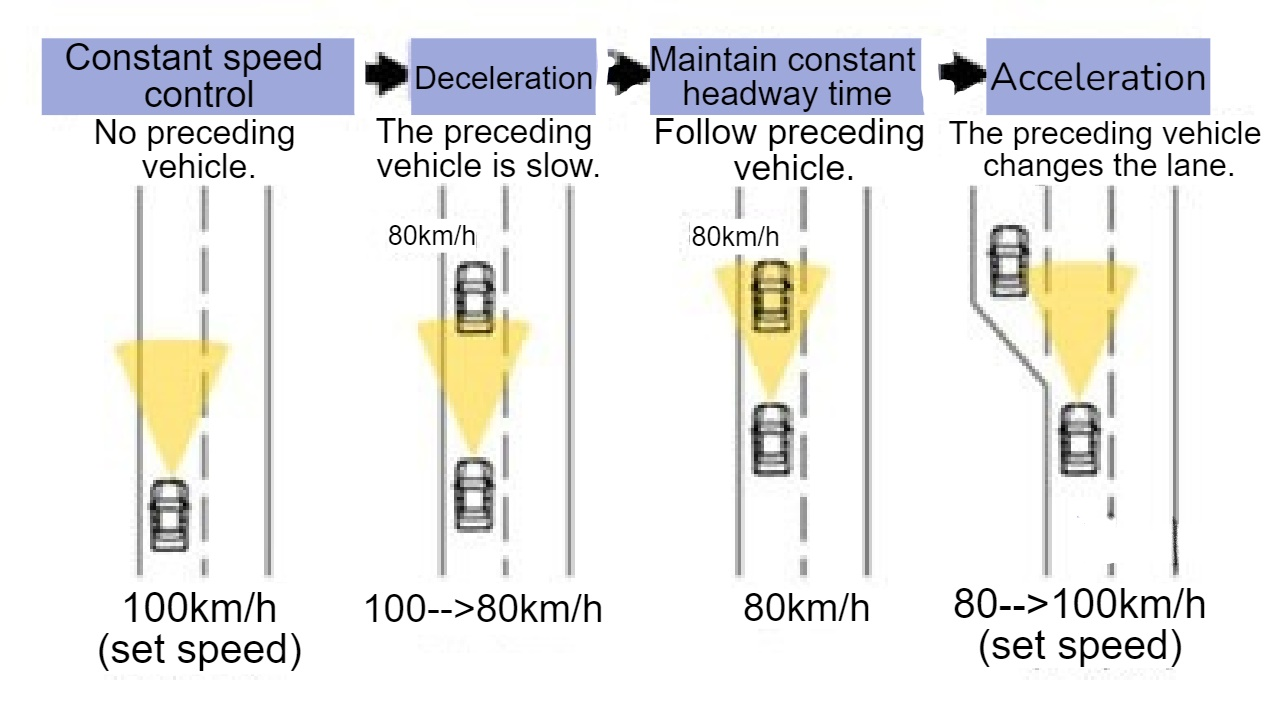
\includegraphics[width=1\textwidth]{Working of ACC.jpg}
    \caption{Working of ACC \cite{Automated}.}
    \label{fig:Working of ACC}    
\end{figure}
\\
\subsection{\fontsize{12}{12}\selectfont{Remote and Autonomous Controlled Robotic Carbased on Arduino with Real Time Obstacle Detection and Avoidance}}
In this system, they design and implement a robotic car regarding hardware, software, and communication environments and detect in real time an obstacle to avoid it. In the implementation of the system, it consists of an Arduino UNO, an HC-06 Bluetooth module, an Arduino motor shield, a DC motor, an ultrasonic sensor HC-SR04, a PIR sensor, a buzzer, a 9V battery, and an Android application. The robotic car consists of two modes: user control and automatic mode. The user can control the robot's basic movements back and forth, right-left rotation, and stop-motion, or put the robotic car in automatic mode to let the car drive its own way, so it can flee from an obstacle and also detect live objects.
\\
\begin{figure}[H]
    \centering
    \graphicspath{ {./images/} }
    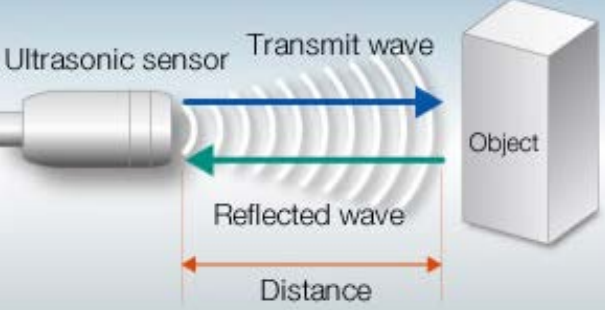
\includegraphics[width=1\textwidth]{Ultrasonic Sensor working principle.png}
    \caption{Ultrasonic Sensor working principle \cite{Robotic}.}
    \label{fig:Ultrasonic Sensor working principle}
    
\end{figure}
The HC-SR04 ultrasonic sensor uses sonar to calculate the distance between the robotic car and the obstacle. It measures between 2 and 400 cm. In Figure (\ref{fig:Ultrasonic Sensor working principle}), it shows the ultrasonic sensor's working principle. If the obstacle is a human, the red LED and buzzer sound will activate. It calculates the shortest distance that can be avoided. If the obstacle is an inanimate entity, it calculates the shortest distance that can be avoided. Furthermore, when the robot reaches the cliff, it perceives the abyss and stops itself\cite{Robotic}. 
\\
\subsection{\fontsize{12}{12}\selectfont{Vision-Based Adaptive Cruise Control Using Pattern Matching}}

This system uses image processing algorithms to detect vehicles and determine range using a single camera. This is done by detecting the fiducial marker which is one of the general signs of cars such as (number plate, rear windshield or tail lights) and when detecting the size and direction the fiducial marker is used to calculate the geometric range.
It works by matching patterns by searching an image for a predefined template It uses normalize cross-correlation to find a template in an image. The underlying algorithm for detecting a vehicle's progress involves the set of a template of the target vehicle with different scales and orientations under different environmental conditions\cite{PatternMatching}.
\\

\begin{figure}[H]
    \centering
    \graphicspath{ {./images/} }
    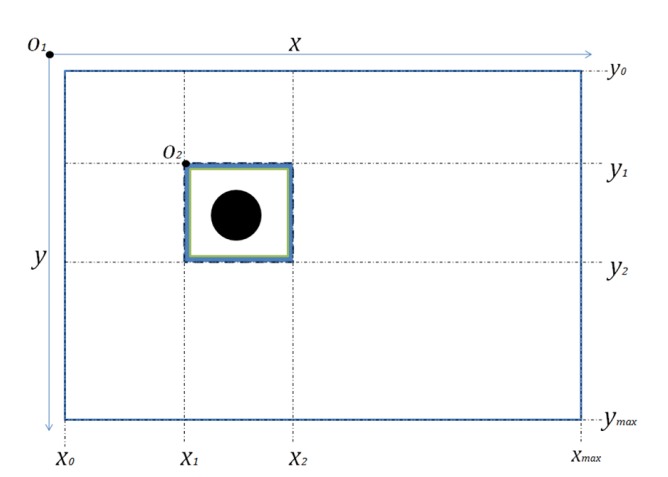
\includegraphics[width=1.09\textwidth,height=.5\textheight]{related.png}
    \caption{Adaptive cropping uses previous vehicle location to restrict ROI \cite{PatternMatching}.}
    \label{fig:mesh1}
\end{figure}


\subsection{\fontsize{12}{12}\selectfont{Analysis of Existing Systems}}
 
 The fundamental issue in the first study is that the ACC is unaware of other cars' movements. The drivers must maintain constant awareness. The expense of designing ACC systems nowadays is one of the most difficult difficulties. The ACC does not drive your automobile for you, and it cannot be utilized in crowded places. Because the object is more than three meters away and has a reflective surface at a shallow angle, the sound will be too small to reflex back to the sensor.
 
 In the second study, they operate the vehicle using components similar to ours and an application. The contrast is that they just identify the obstruction. If an impediment is in front of the automobile, they do nothing to slow it down or speed it up. As a result, we have an edge.

Finally, in the third study, it is difficult in practice to identify a generic fiducial marker that can be accurately detected at medium-to-long distances (more than 30 meters). For example, number plates often come in different shapes and are too small to be accurate. identified and measured by a camera with reasonable resolution.



%--[chapter3:METHODS AND MATERIALS]------------------------------------------------------------------------------------------------------------------------
\chapter{METHODS AND MATERIALS}
\section{\fontsize{12}{12}\selectfont{System Design and Components}}
\subsection{\fontsize{12}{12}\selectfont{Block Diagram}}
In Figure (\ref{fig:Block Diagram}), it shows the block diagram of ACC system.
\begin{figure}[H]
    \centering
    \graphicspath{ {./images/} }
    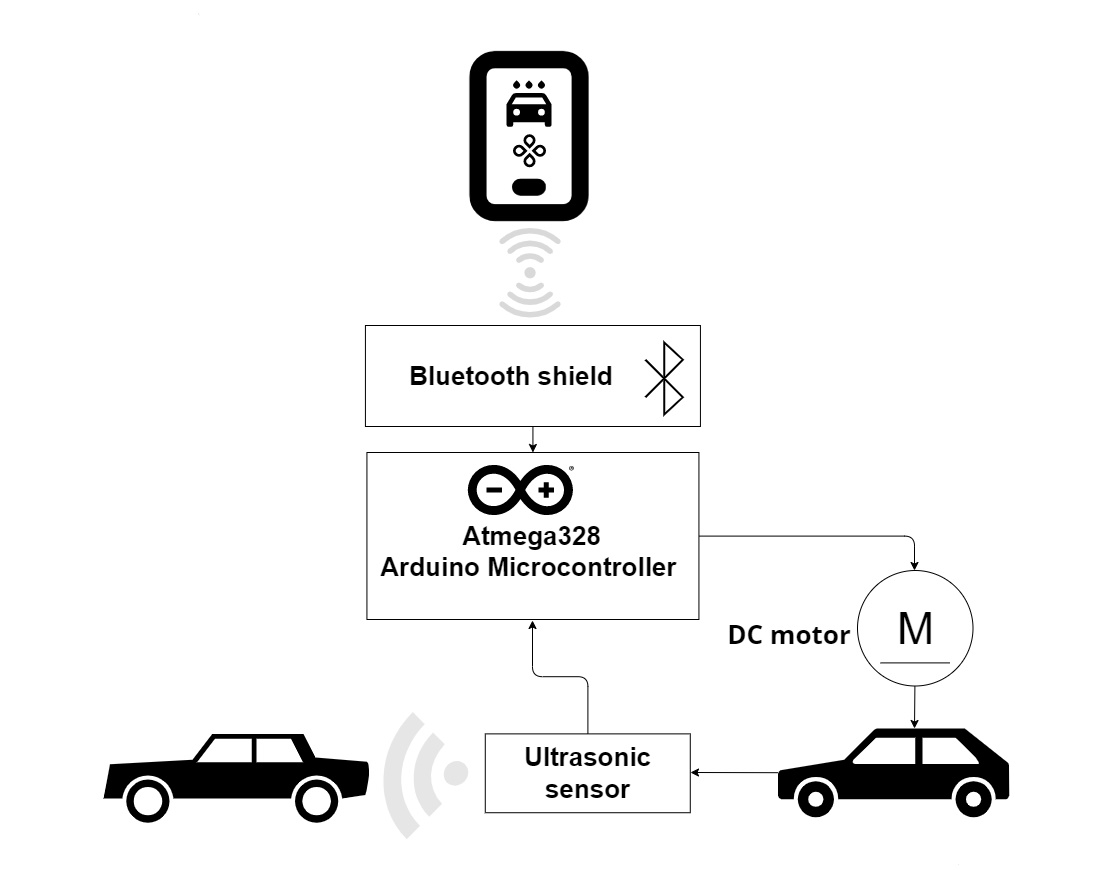
\includegraphics[width=1\textwidth]{ACC block diagram.jpg}
    \caption{Block Diagram}
    \label{fig:Block Diagram}
\end{figure}
\break
\subsection{\fontsize{12}{12}\selectfont{Hardware Components}}

{ \textbf{Micro-controller:}} 



Table (\ref{tab:micro}) shows a comparison between the most important types of Arduino micro-controller based on several elements, in order to determine the best and most suitable type for the project.

%------------------------------------Ardunio types
\begin{table}[H]
\begin{center}
\caption{Arduino microcontrollers specification 
\cite{Arduino1},\cite{Arduino2}. }
\label{tab:micro}  
\begin{tabular}{|p{1.7cm}  |p{2.3cm}  |p{1.2cm}  |p{2cm}
|p{1.5cm} |p{1.3cm}  |p{1.4cm}   |p{1cm}|}
\hline
\textbf{Arduino Name} 
& \textbf{Processor}
& \textbf{CPU speed}
& \textbf{Operating Voltage(V)}
& \textbf{Digital IO/PWM}
& \textbf{Analog pins}
& \textbf{Flash memory(KB)}
& \textbf{Price
(ILS)} \\ 

\hline

\textcolor{bb}{Uno}	& \textcolor{bb}{ATmega328} 
 & \textcolor{bb}{16MHz}  & \textcolor{bb}{7-12}	
  & \textcolor{bb}{14/6}	&\textcolor{bb}{6}	
   &\textcolor{bb}{32} &\textcolor{bb}{50.0} \\\hline

Leonardo &ATmega32u4 &16MHz	&5	&20/7	&12	&32	&50.0 \\\hline

Mega2560 	&ATmega2560	&16MHz	&5	&54/15	&16	&256	 &95.0\\\hline

Nano	 &ATmega328	&16MHz	&5	&14/6	&8	&32	&35.0\\\hline

Mini pro	 &ATmega328	&16MHz	&5	&14/6	&8	&32	&35.0 \\\hline

Lilypad	&ATmega328V	&8MHz	&2.7-5.5 	&14/6	&6	&16	&50.0\\\hline

\end{tabular}
\end{center}  
\end{table}

Depending on the attached table and comparing with the features we need in our project like number of inputs we need, size and price.We will use Arduino (UNO/ATmega328) in our project.\\

%............................Arduino(UNO/ATmega328)............................
{\textbf{Arduino(UNO/ATmega328):}} \\

The Arduino UNO is categorized as a micro-controller that uses the ATmega328 as a controller of it. It is a simple electronic device that is designed for easy use, it is able to receive different types of input signals and resend them as preferred outputs. This board includes 14 digital I/O pins, 6 of them possible to be applied for PWM (Pulse Width Modulation) yields, there are 6 Analog pins, USB connection, a power jack, in addition to a reset button, all are included there, in other words the Arduino contains everything needed for a control device. Also, it can be connected to a computer via an USB cable or Bluetooth module\cite{Arduino}.


\begin{figure}[H]
    \centering
    \graphicspath{ {./images/} }
    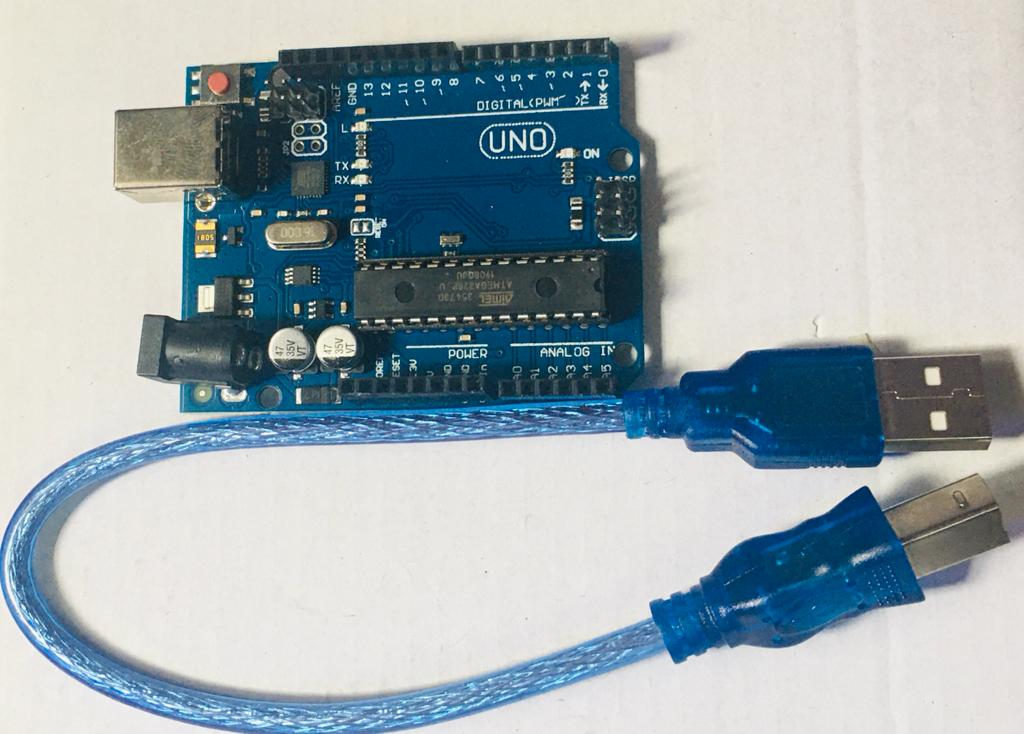
\includegraphics[width=8cm, height=5cm]{uno1.jpg}
    \caption{Arduino(UNO/ATmega328)}
    \label{fig:mesh1}
\end{figure}
%.......................Ultrasonic Sensor.................
\textbf{{Ultrasonic Sensor:}}\\


Ultrasonic sensors measure distance using ultrasound, the principle of ultrasonic sensors is that the transmitter part sends sound signals with a frequency of more than 18 kHz into the air at a speed of 344 m/s (at about 20°C) and then the device receives the reflected signals from the target. Ultrasound sensors measure the distance to a target by measuring the time between emission and reception. This can be done up to four meters\cite{UltrasonicSensor}.\\

\textbf{Ultrasonic Sensor specifications:}\\

•	Working Voltage: 5V(DC).\\
•	Static current: Less than 2mA.\\ 
•	Output signal: Electric frequency signal, high level 5V, low level 0V.\\ 
•	4Sensor angle: Not more than 15 degrees.\\
•	Detection distance: 2cm-450cm.\\ 
•	High precision: Up to 0.3cm.\\


\begin{figure}[H]
    \centering
    \graphicspath{ {./images/} }
    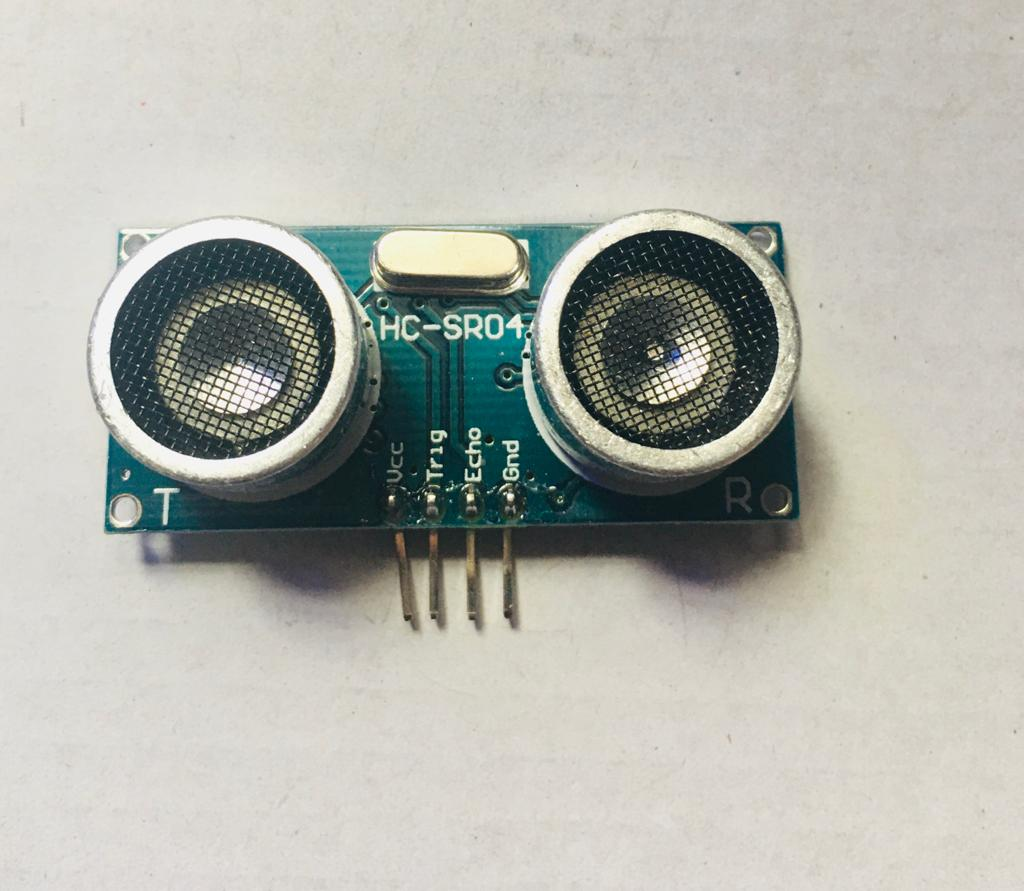
\includegraphics[width=8cm, height=5cm]{ultra.jpg}
    \caption{ Ultrasonic Sensor}
    \label{fig:mesh1}
\end{figure}
\bigskip
%....................HC-06 Bluetooth module:....................

\textbf{{ HC-06 Bluetooth module:}}\\

Bluetooth is a wireless device that allows two micro-controllers or systems to transmit or receive TTL data over short distances via Bluetooth without connecting a serial cable to computer. It is one of the cheapest and the most flexible way to transfer wireless data compared to other methods. HC-06 uses frequency hopping to spread spectrum technique (FHSS) to avoid interference with other devices and to have full duplex transmission. The device works on the frequency range from 2.402 GHz to 2.480GHz\cite{Bluetooth}.

HC-06 Bluetooth module in our project will be the link to data exchange between the mobile application and the Arduino micro-controller.\\

\textbf{HC-06 Bluetooth module specifications:}\\

•	Default Baud Rate: 9600,8,1, n.\\
•	Built in antenna.\\
•	Coverage up to 30ft.\\
•	Operating voltage: 3.3V\\
•	Default Baud Rate: 9600,8,1, n.\\
•	Signal coverage: 30ft.\\
•	Item size: 4.3 * 1.6 * 0.7cm\\
•	Item weight: 3g.\\

\begin{figure}[H]
    \centering
    \graphicspath{ {./images/} }
    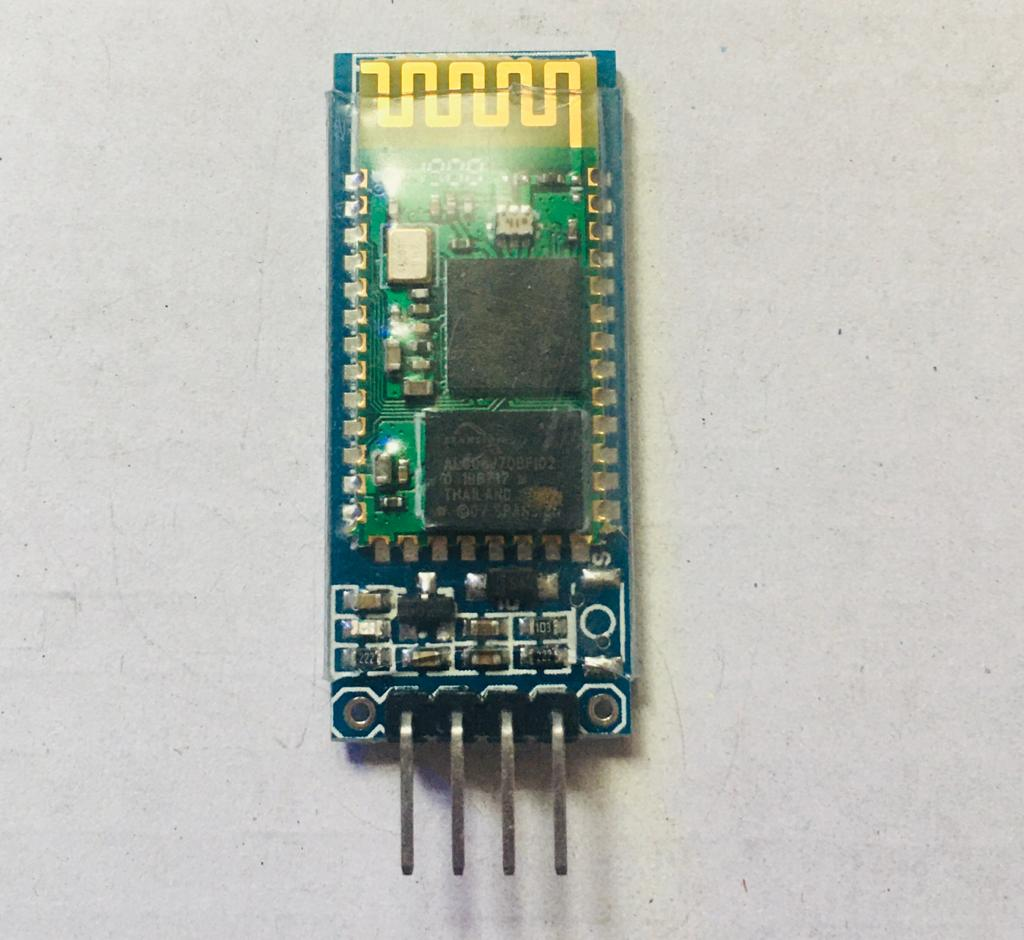
\includegraphics[width=8cm, height=5cm]{blutooth.jpg}
    \caption{ HC-06 Bluetooth module}
    \label{fig:mesh1}
\end{figure}
\bigskip
\bigskip
\bigskip
\bigskip
\bigskip
\bigskip
\bigskip
\bigskip
\bigskip
\bigskip
\bigskip
\bigskip
\bigskip
\bigskip
\bigskip
\bigskip
%..........Motor Drive Module Board (L298N Dual H-Bridge):..................

\textbf{{Motor Drive Module Board (L298N Dual H-Bridge):}}\\

The L298N is a module for motors that used in controlling motor speed and direction. This Motor Driver is designed and developed based on L293D IC. L293D is a 16 Pin Motor Driver IC. This is designed to provide bidirectional drive currents at voltages from 5 V to 35 V \cite{motordriver}. In our project the driver used to connect DC-motor of the prototype-car to control the directions and speed of the prototype-car according to Pulse with Modulation (PWM).\\

\textbf{Motor driver specifications:}\\

•	Chip: L298N.\\ 
•	Logical voltage: 5V.\\
•	Drive voltage: 5V-35V.\\
•	Logical current: 0mA-36mA.\\
•	Drive current: 2A (MAX single bridge).\\
•	Storage temperature: -20 to +135.\\
•	Max power: 25W.\\
•	Weight: 30g.\\


\begin{figure}[H]
    \centering
    \graphicspath{ {./images/} }
    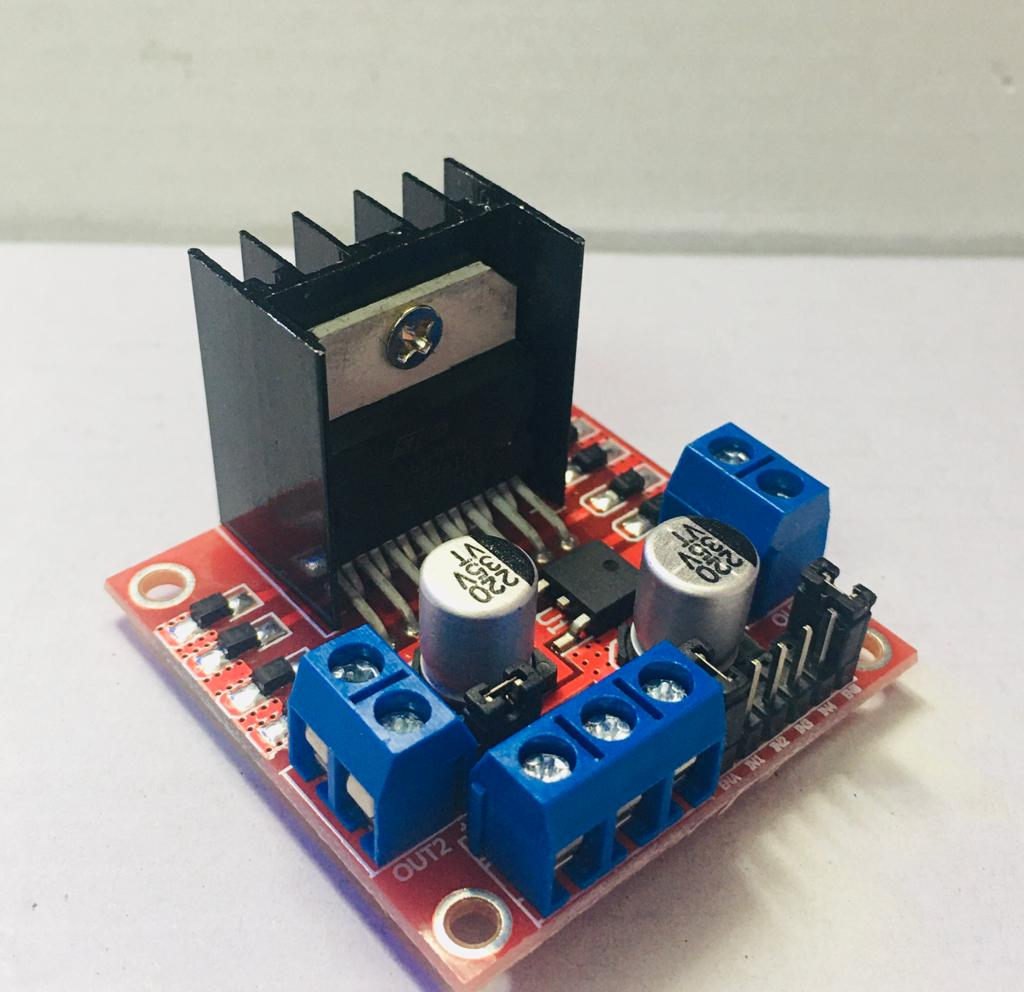
\includegraphics[width=8cm, height=5cm]{driver.jpg}
    \caption{ Motor Drive Module Board (L298N Dual H-Bridge)}
    \label{fig:mesh1}
\end{figure}

%..........Car with 4 DC Geared Motor:..................

\textbf{{ Car with 4 DC Geared Motors:}}\\

The vehicle that will be used in our project it is a suspension damping vehicle with four wheels and two layers of 3mm thick acrylic plates as the main structure. In addition, there are four rubber tires with a diameter of 65 mm and four powerful magnetic drivers with a shock mitigation system. It is lightweight and suitable for all types of terrain. This unique cushioning ability ensures that the car is not easily damaged. The working voltage is 3V-9V, working current is 400mA and the maximum motor voltage is 6VDC, the tire speed can reach 90 rpm when there is no load. \\

\textbf{{Geared Motor specifications:}}\\

•	Operating voltage: 3V-12V.\\
•	Load current: 70mA(250mA MAX).\\


\begin{figure}[H]
    \centering
    \graphicspath{ {./images/} }
    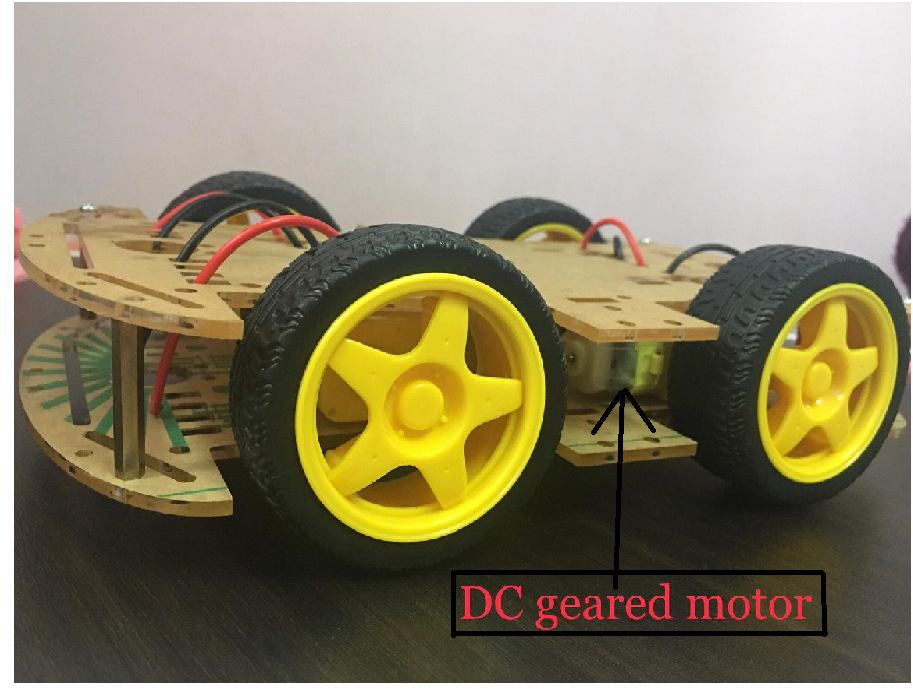
\includegraphics[width=8cm, height=5cm]{cardcmotor.PNG}
    \caption{ Car with 4 DC Geared Motors}
    \label{fig:mesh1}
\end{figure}

Figure (\ref{fig:car}) shows an initial image of the car as it appears in its final form.
\begin{figure}[H]
    \centering
    \graphicspath{ {./images/} }
    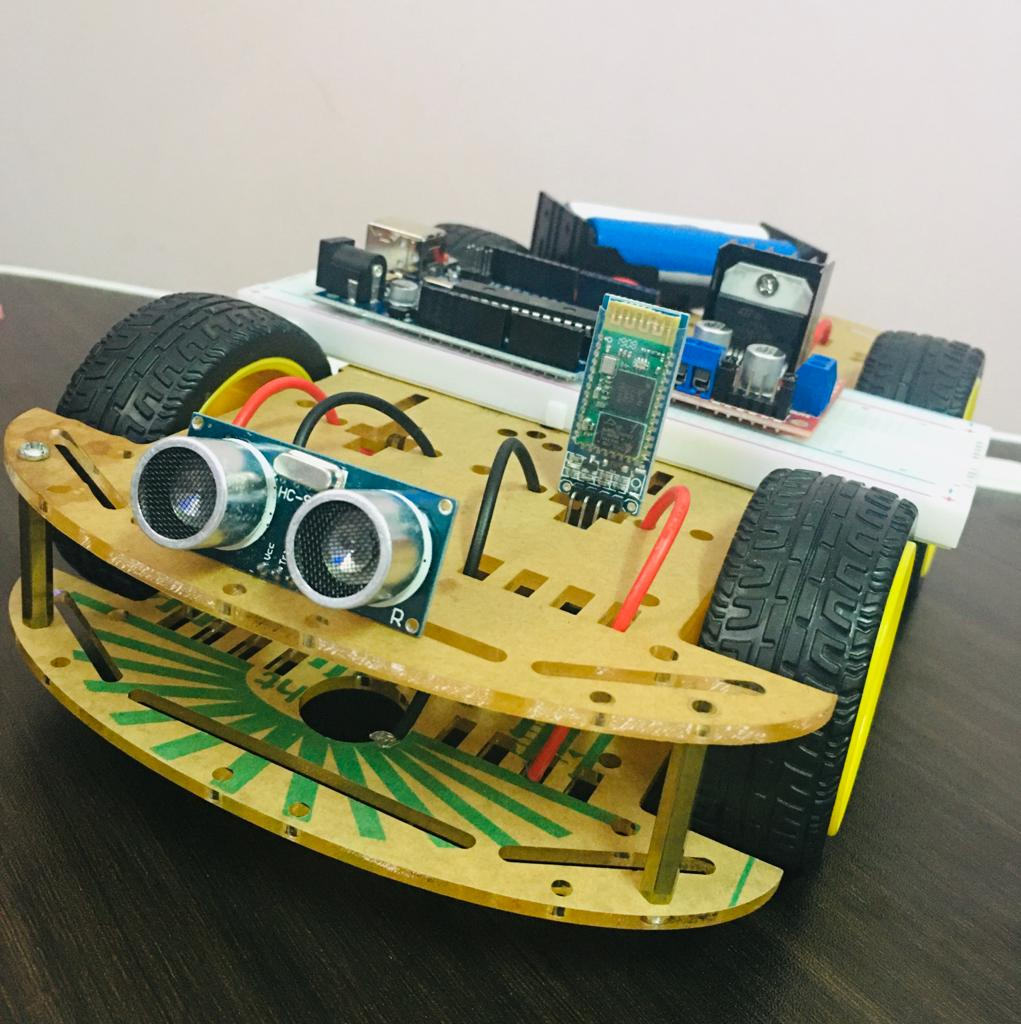
\includegraphics[width=8cm, height=5cm]{prototype.jpg}
    \caption{The prototype-car}
    \label{fig:car}
\end{figure}
%.................Power supply.....................................
\textbf{{Power supply:}}\\

The battery is the power source of both the motors and the microcontroller. The single battery of type lithium-ion give a 3.7V and is rechargeable through the charger attached to the picture in figure (\ref{fig:wires1}).\\

\begin{figure}[H]
    \centering
    \graphicspath{ {./images/} }
    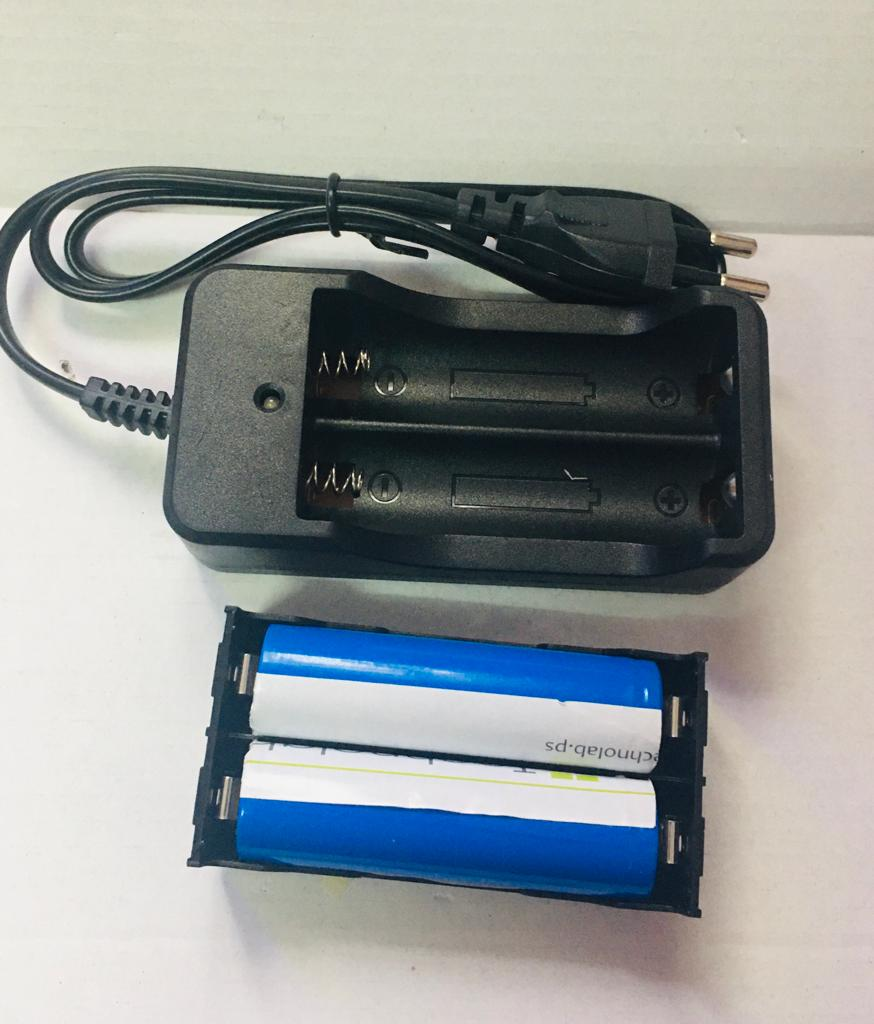
\includegraphics[width=8cm, height=5cm]{power.jpg}
    \caption{Power supply}
    \label{fig:Power}
\end{figure}
%............................Wires...............
\textbf{{Wires:}}\\

Figure (\ref{fig:wires1}) and Figure (\ref{fig:wires2})  shows the wires that we need for connections in our project, female to female jumper wires and female to male jumper wires.

\begin{figure}[H]
    \centering
    \graphicspath{ {./images/} }
    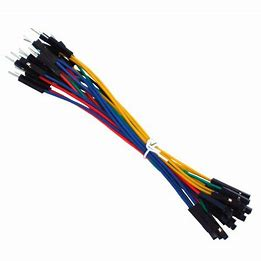
\includegraphics[width=8cm, height=5cm]{FemaletoMalejumperwire.jpg}
    \caption{Female to Male jumper wires}
    \label{fig:wires1}
\end{figure}
\begin{figure}[H]
    \centering
    \graphicspath{ {./images/} }
    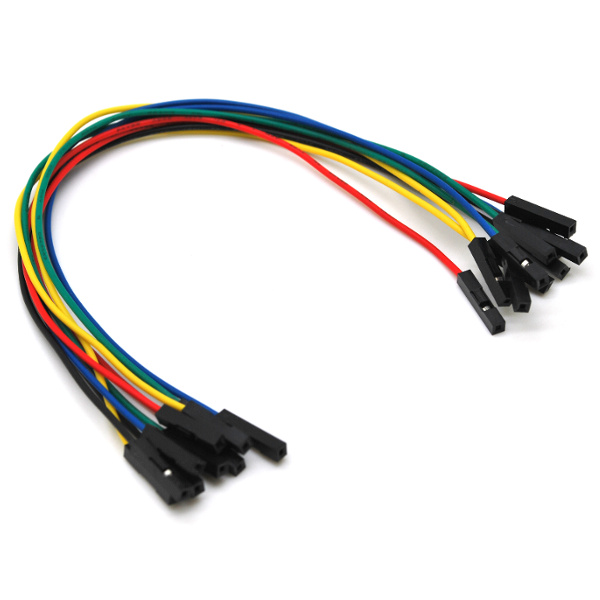
\includegraphics[width=8cm, height=5cm]{FemaletoFemaleJumperWires.jpg}
    \caption{Female to Female Jumper Wires}
    \label{fig:wires2}
\end{figure}
\bigskip
\bigskip
%.................................Breadboard...........................
\textbf{{ Breadboard:}}\\

Figure (\ref{fig:Breadboard}) shows the breadboard that we will use in our project,it helps to make connections without the need for welding.\\

\begin{figure}[H]
    \centering
    \graphicspath{ {./images/} }
    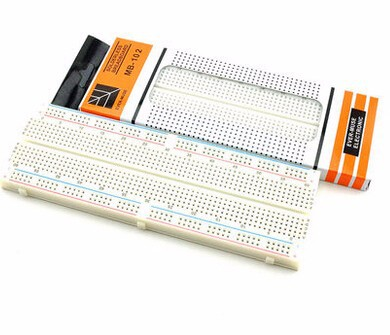
\includegraphics[width=8cm, height=5cm]{Breadboard.jpg}
    \caption{Breadboard}
    \label{fig:Breadboard}
\end{figure}
%.............








\section{\fontsize{12}{12}\selectfont{{Design Specifications, Standards and Constraints}}}
\subsection{\fontsize{12}{12}\selectfont{Specifications:}}
\renewcommand{\theenumi}{\roman{enumi}}%
\begin{enumerate}
  \item Set the car speed using a mobile app and keep a consistent car speed.
  \item Keep enough space between the driver's car and other cars.
  \item Turn on and off the ACC system using a mobile app.
  \item Turn on and off the car and control the direction of it using a mobile app.
  \item Contain an alert for the driver when the lead car exceeds the limit of distance between them.
\end{enumerate}

\subsection{\fontsize{12}{12}\selectfont{Constraints:}}
The components were not readily available in our city, and obtaining them required some effort. The Bluetooth connection model's maximum range is 9 meters, so the capacity to manage the automobile is limited. External circumstances caused the hardware parts to fail, requiring us to purchase the parts (Arduino, drivers) again, increasing the project cost. Because it is costly to cover all of the pieces required to achieve all of the functions in ADAS, we have picked one of these features.


\subsection{\fontsize{12}{12}\selectfont{Standards:}}
The most important standards used in the components used in our project:
\begin{itemize}
  \item HC-06 Bluetooth Module: IEEE 802.15.1 standardized protocol.  
  \item Arduino Uno:
  \begin{itemize}
  \item UART:universal asynchronous receiver-transmitter, is one of the most used
   device-to-device communication protocols . 
  \item I2C:stands for Inter-Integrated Circuit, it is a bus interface connection
   protocol incorporated into devices for serial communication specially designed
    for microcontrollers.
  \item SPI:stands for Serial Peripheral Interface, is an interface bus commonly
   used to send data between microcontrollers and small peripherals. 
\end{itemize}
  
  \item lithium-ion battery: ISO 26262 safety standard for lithium-ion battery. 
\end{itemize}


\section{\fontsize{12}{12}\selectfont{Design Alternatives}}
In the alternatives section, we presented three designs that evolved from the first concepts to the final product. We'll try to explain why the other designs failed and how we came up with this solution in this part.
\begin{itemize}
\item The first design, which had our basic first idea, the use of distance sensors, was key to this system in that we are going to construct our controlling unit to control the complete system by employing Ultrasonic Range Finder-LV-MaxSonar-EZ1. This design had a number of flaws, including that there were better options depending on the price. We saved money by using the Ultrasonic Sensor Module HC-SR-04 instead of the Ultrasonic Range Finder-LV-MaxSonar-EZ1.

 \item The second design, we tried to use flutter for the android application, but we opted to stick with Java since we were familiar with it and because flutter documentation and resources were not as widely available online as Java. As a result, if we face any problems, an unusual bug, or an issue in our application, it may be more difficult to fix than with Java.

 \item In the thired design, there are two types of microcontrollers to employ that the Arduino and the Raspberry Pi. However, we chose the Arduino Uno since it is low-power, less expensive than the Raspberry Pi, and the digital and analog ports provide a wide range of communication, so the vast number of I/O pins allows you to connect various sensors and components.
 
  \item In the fourth design, while there are numerous different connection technologies today, Bluetooth and Wi-Fi are the two most widely used. Compared to Wi-Fi, Bluetooth devices use less electricity. The Bluetooth model was created with minimal energy usage in mind. And Bluetooth gadgets are typically less expensive. We chose the Bluetooth HC-06.
\end{itemize}

The final design corrects the flaws in the earlier designs. to complete the task and meet our expectations in terms of cost and timeliness.
\section{\fontsize{12}{12}\selectfont{System Analysis and Optimization}}

%----------------------------------------------------------------------------------------------------------------------------------------------------------
\subsection{\fontsize{12}{12}\selectfont{ACC flow chart:}}
In Figure (\ref{fig:ACC flow chart}), it shows the flow chart of ACC system.
\begin{figure}[H]
    \centering
    \graphicspath{ {./images/} }
    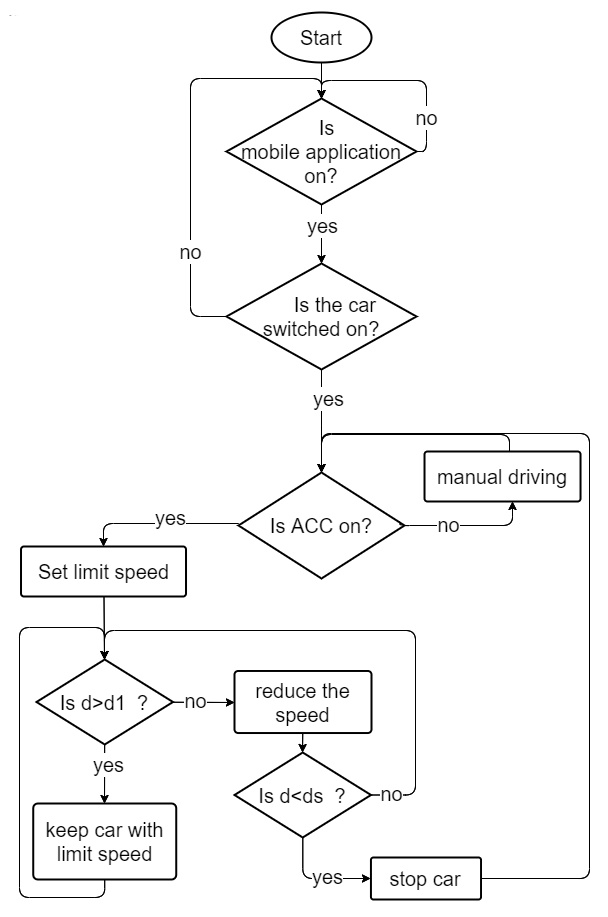
\includegraphics[width=0.8\textwidth,height=16.5cm]{ACC flow chart.jpg}
    \caption{Flow chart}
    \label{fig:ACC flow chart}
\end{figure}
d is distance between the car and the front object.\\
d1 is a varying distance with a value depending on the speed of the car.\\
ds is the threshold distance to stop the car.\\


%----------------------------------------------------------------------------------------------------------------------------------------------------------
\subsection{\fontsize{12}{12}\selectfont{ACC use case:}}
In Figure (\ref{fig:useCase}), it shows the use case of ACC system.
\begin{figure}[H]
    \centering
    \graphicspath{ {./images/} }
    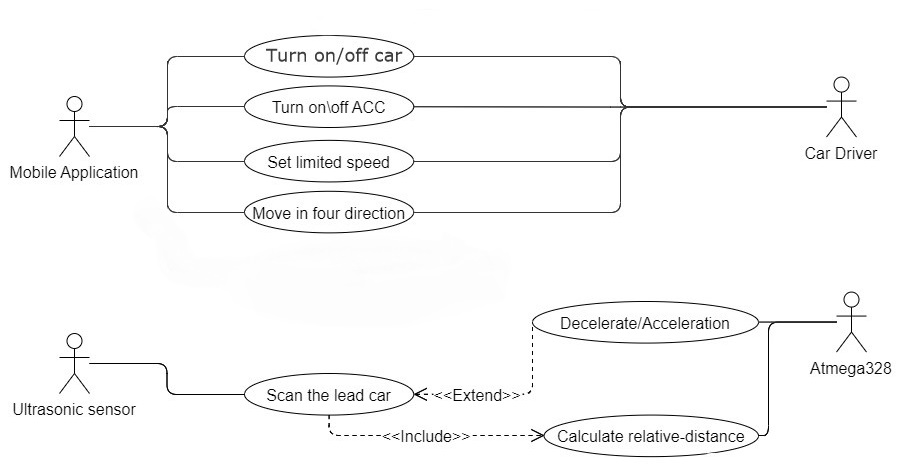
\includegraphics[width=1\textwidth]{ACC use case .jpg}
    \caption{Use case}
    \label{fig:useCase}
\end{figure}
%--------------------------------------------------------------------------------------------------------------------------[USE CASE TABLE]----------------
\subsection{\fontsize{12}{12}\selectfont{ACC use case tables:}}
%------------------------------------use case 1
\begin{table}[H]
\begin{center}
\caption{Use case 1}
\label{tab:use3} 
\begin{tabular}{|p{3cm}|p{11cm}|}
\hline
\textbf{Use Case 1} & \textbf{Turn on/off the car}\\ 
\hline
Actor(s)&The Driver and Mobile Application.\\\hline
Type&Primary\\\hline
Description&Enable the driver to turn on or off the car.\\\hline
Pre-condition&Connect to Bluetooth successfully.\\\hline
Post-condition&Enables the driver to choose between using ACC while driving or manual driving.\\\hline
\end{tabular}
\end{center}  
\end{table}
%------------------------------------use case 2
\begin{table}[H]
\begin{center}
\caption{Use case 2}
\label{tab:use4}
\begin{tabular}{|p{3cm}|p{11cm}|}
\hline
\textbf{Use Case 2} & \textbf{Turn on/off ACC system.}\\ 
\hline
Actor(s)&The Driver and Mobile Application.\\\hline
Type&Primary\\\hline
Description&Enable the driver to turn on or off ACC system.\\\hline
Pre-condition&The car is turn on.\\\hline
Post-condition&Set the car speed using a mobile app and keep the speed in limit.\\\hline
\end{tabular}
\end{center}  
\end{table}
%------------------------------------use case 3
\begin{table}[H]
\begin{center}
\caption{Use case 3}
\label{tab:use5}
\begin{tabular}{|p{3cm}|p{11cm}|}
\hline
\textbf{Use Case 3} & \textbf{Set limit speed
}\\ 
\hline
Actor(s)&The Driver and Mobile Application.\\\hline
Type&Primary\\\hline
Description&Set the car speed.\\\hline
Pre-condition&The ACC is turn on.\\\hline
Post-condition&Keep car speed in limit.\\\hline
\end{tabular}
\end{center}  
\end{table}
%------------------------------------use case 4
\begin{table}[H]
\begin{center}
\caption{Use case 4}
\label{tab:use6}
\begin{tabular}{|p{3cm}|p{11cm}|}
\hline
\textbf{Use Case 4} & \textbf{Move the car in four direction}\\ 
\hline
Actor(s)&The Driver and Mobile Application.\\\hline
Type&Primary\\\hline
Description&The user can select which direction to go in, like forward, back, left, or right.\\\hline
Pre-condition&The car is turned on and the limit speed is selected.\\\hline
Post-condition&Shows car’s actual speed and position on a mobile app.\\\hline
\end{tabular}
\end{center}  
\end{table}
%------------------------------------use case 5
\begin{table}[H]
\begin{center}
\caption{Use case 5}
\label{tab:use8}
\begin{tabular}{|p{3cm}|p{11cm}|}
\hline
\textbf{Use Case 5} & \textbf{Calculate relative-distance}\\ 
\hline
Actor(s)&Atmega328\\\hline
Type&Secondary\\\hline
Description&Calculate the relative distance between the driver's car and the scanned distance by the ultrasonic sensor.\\\hline
Pre-condition&The ultrasonic sensor scans the lead car.\\\hline
Post-condition&Decelerate/Acceleration the car.\\\hline
\end{tabular}
\end{center}  
\end{table}
%------------------------------------use case 6
\begin{table}[H]
\begin{center}
\caption{Use case 6}
\label{tab:use10}
\begin{tabular}{|p{3cm}|p{11cm}|}
\hline
\textbf{Use Case 6} & \textbf{Scan the lead car}\\ 
\hline
Actor(s)&Ultrasonic sensor\\\hline
Type&Secondary\\\hline
Description&The ultrasonic sensor scans the distance between the driver's car and the lead car.\\\hline
Pre-condition&The ACC system is activated.\\\hline
Post-condition&Calculate relative-distance\\\hline
\end{tabular}
\end{center}  
\end{table}
%------------------------------------[cases]---------------------------------------------------------------------------------------------------------------
\subsection{\fontsize{12}{12}\selectfont{ACC Sequence Diagrams:}}

\begin{figure}[H]
    \centering
    \graphicspath{ {./images/} }
    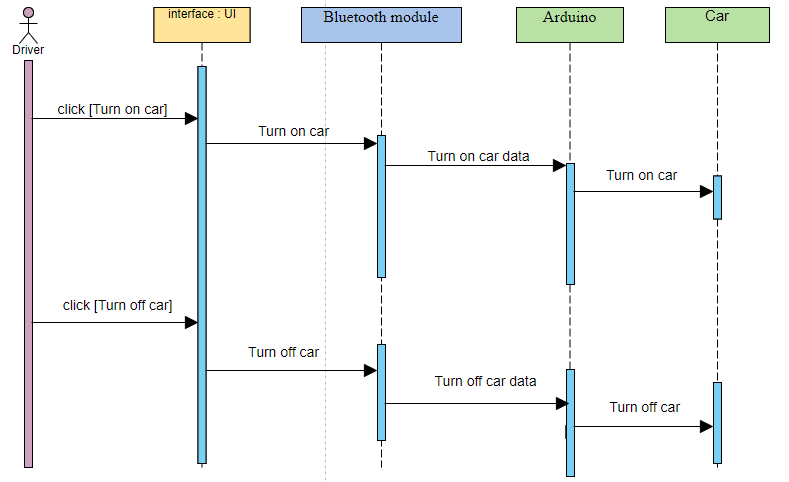
\includegraphics[width=1\textwidth]{case3.png}
    \caption{Turn on-off car sequence }
    \label{fig:mesh1}
\end{figure}
\begin{figure}[H]
    \centering
    \graphicspath{ {./images/} }
    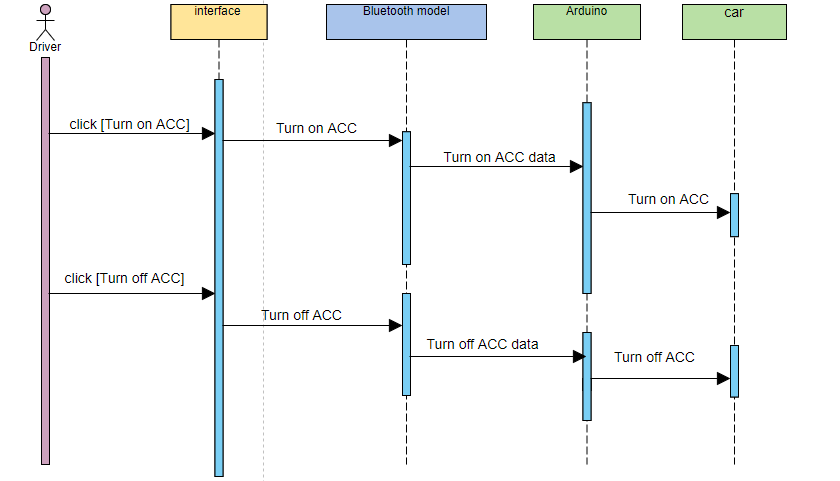
\includegraphics[width=1\textwidth]{case4.png}
    \caption{Turn on-off ACC sequence}
    \label{fig:mesh1}
\end{figure}

%.........
\begin{figure}[H]
    \centering
    \graphicspath{ {./images/} }
    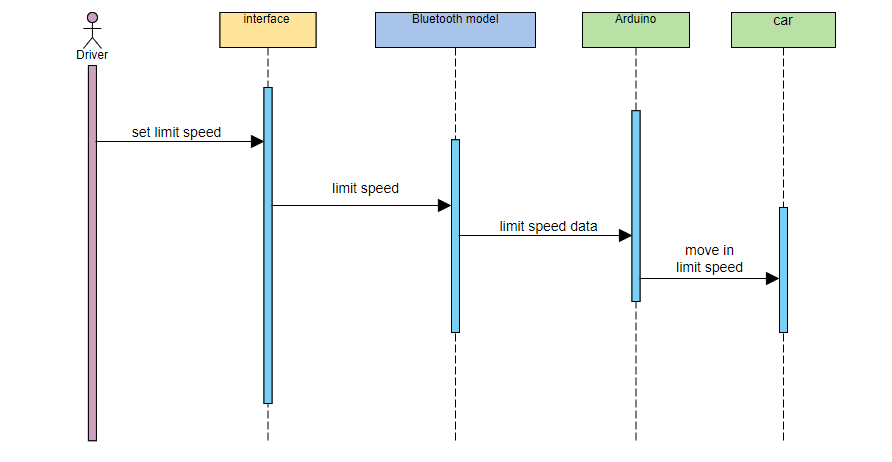
\includegraphics[width=1\textwidth,height=.4\textheight]{case5.png}
    \caption{Set limit speed sequence}
    \label{fig:mesh1}
\end{figure}
%.............
\begin{figure}[H]
    \centering
    \graphicspath{ {./images/} }
    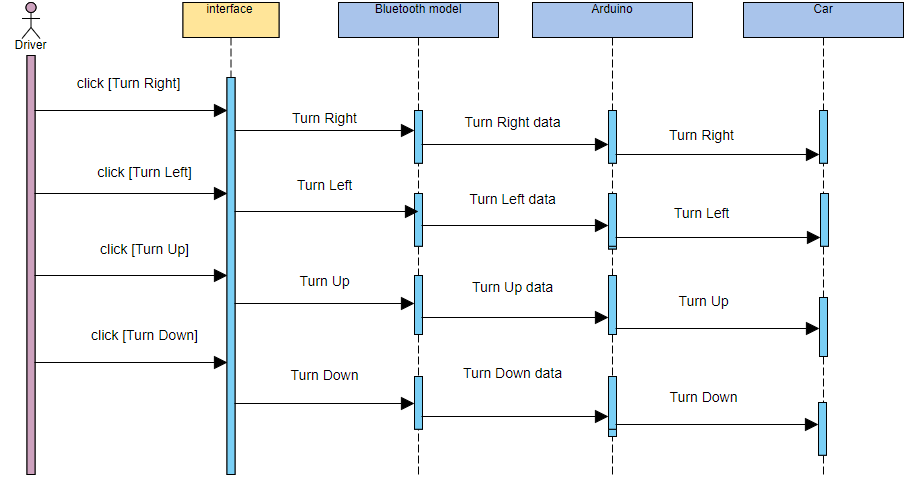
\includegraphics[width=1\textwidth]{case6.png}
    \caption{Move the car in four direction sequence}
    \label{fig:mesh1}
\end{figure}
\begin{figure}[H]
    \centering
    \graphicspath{ {./images/} }
    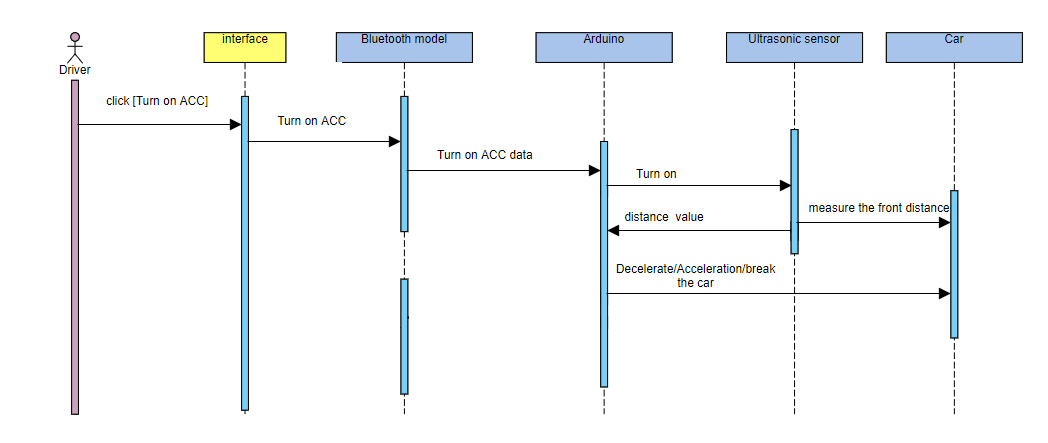
\includegraphics[width=1.05\textwidth,height=.45\textheight]{hard.png}
    \caption{Hardware  sequence}
    \label{fig:mesh1}
\end{figure}
\bigskip
\bigskip
\bigskip
\bigskip
\subsection{\fontsize{12}{12}\selectfont{ACC State Diagram:}}
In Figure (\ref{fig:State}), it shows the State Diagram of  system.
\begin{figure}[H]
    \centering
    \graphicspath{ {./images/} }
    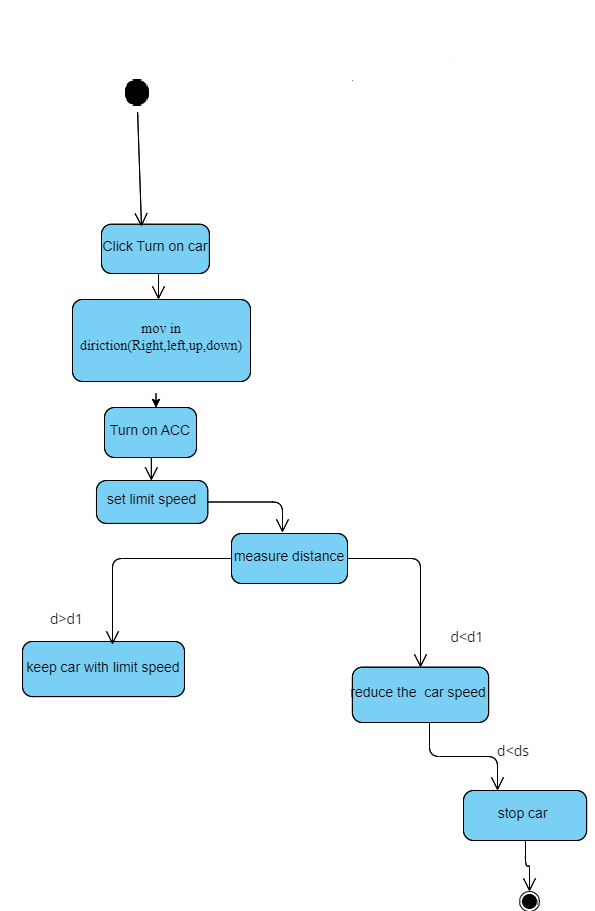
\includegraphics[width=1\textwidth,height=20.5cm]{state diagram (1).png} 
    \caption{ ACC State diagram}
    \label{fig:State}
\end{figure}



\section{\fontsize{12}{12}\selectfont{Simulation and/or Experimental Test}}
In the simulation, we used tools like  tinkercad and Proteus to understand and illustrate connections and to simulate components and understand how each works separately.
\subsection{\fontsize{12}{12}\selectfont{Test Ultrasonic sensor using the  tinkercad simulator.}}
Figure (\ref{fig:Distance}) shows a simulation (using a tinkercad simulator) that we ran on the ultrasonic sensor to make sure that the connections were correct and that the equation used to find the distance is correct.

The formula \textbf{distance = speed*time} is used to calculate the distance. But because the time from the sensor represents the time taken from the wave to travel and then echo back, so we divide the distance by 2, and the equation become:
\textbf{distance =(speed*time)/2} 
and the waves move with sound speed, which is 340m/s, equivalent to 0.034cm/µs 
so, the equation become:\\
\textbf{distance=(0.034cm/µs*time) }also equivalent to \textbf{distance= pulse / 29.387 / 2}\\
which we use in our code where pulse represent the time from echo Pin.


\begin{figure}[H]
    \centering
    \graphicspath{ {./images/} }
    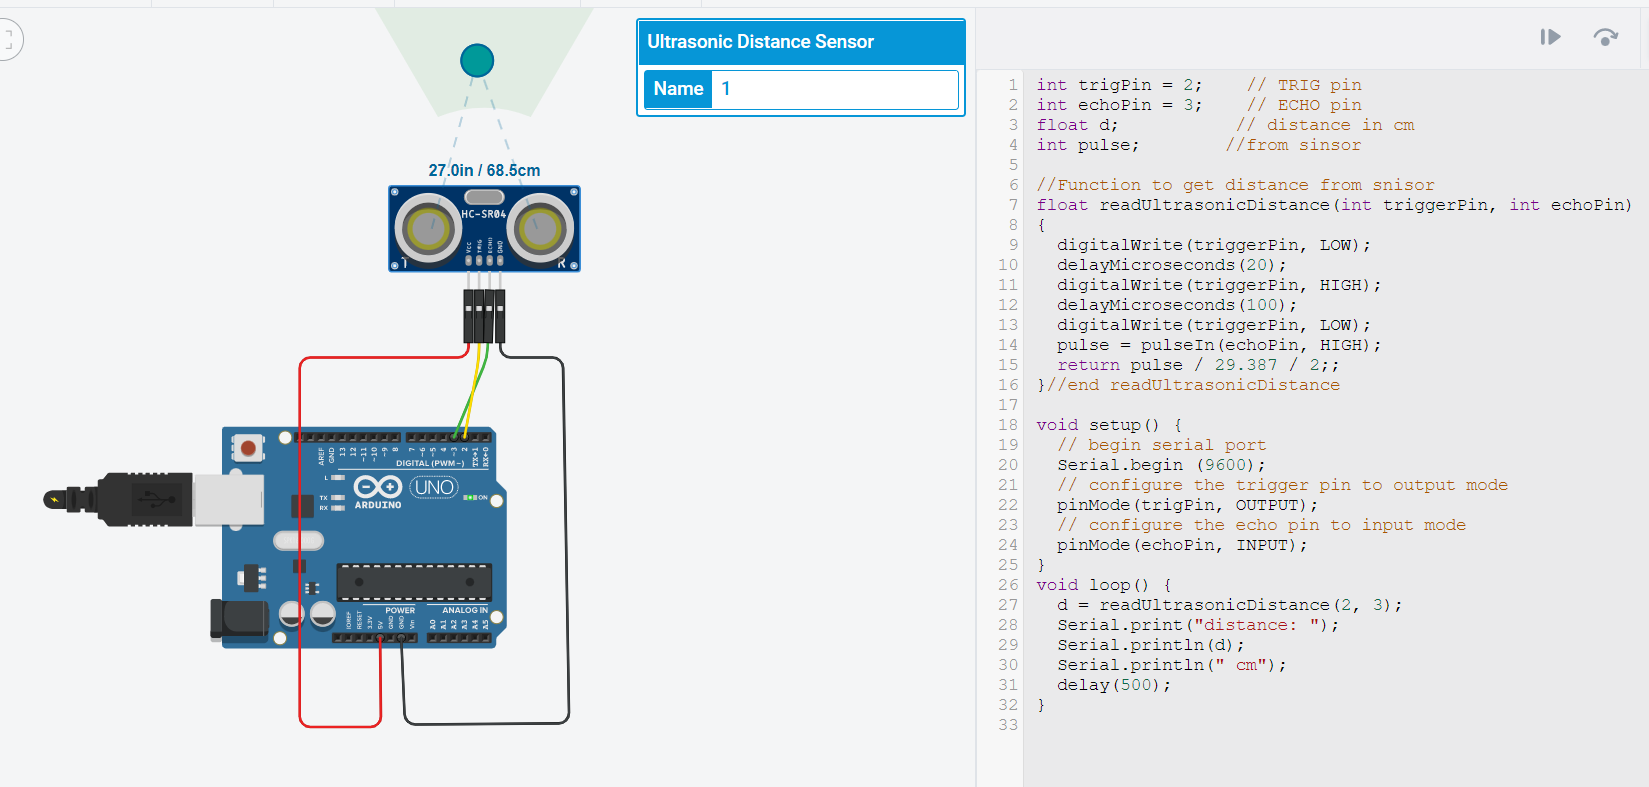
\includegraphics [width=16cm,height=12cm]{Ultra.PNG}
    \caption{Find the distance using an ultrasonic sensor.}
    \label{fig:Distance}
\end{figure}

\subsection{\fontsize{12}{12}\selectfont{Control motor speed according to distance using the tinkercad simulator.}}
Figure (\ref{fig:Speed}) shows a simulation (using a tinkercad simulator) that we ran on the ultrasonic sensor and DC motor to make sure the connections were correct and that the motor's speed was changing according to the measured distance from the sensor.
\begin{figure}[H]
    \centering
    \graphicspath{ {./images/} }
    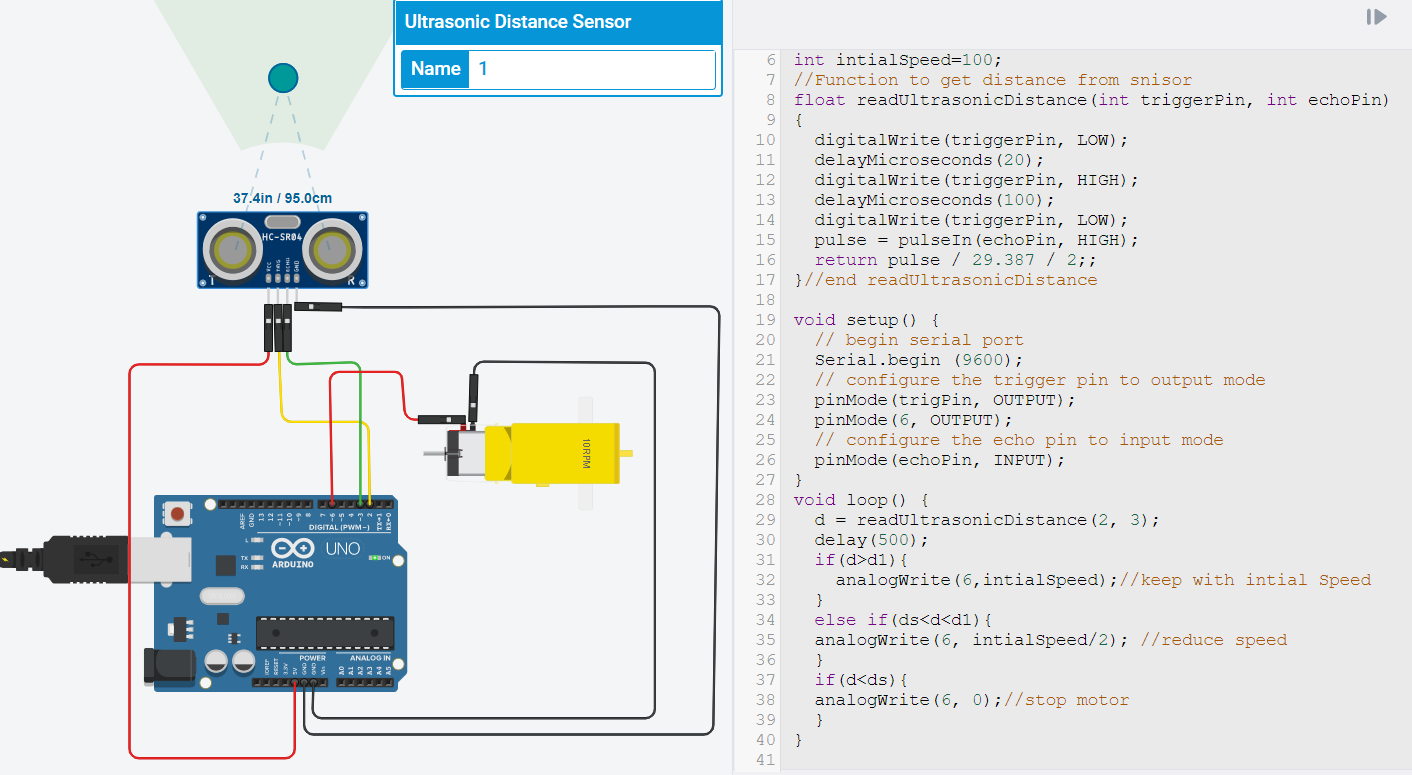
\includegraphics [width=16cm,height=12cm]{motorspeed.PNG}
    \caption{Control motor speed according to distance.}
    \label{fig:Speed}
\end{figure}



\subsection{\fontsize{12}{12}\selectfont{ System connections using the proteus simulator.}}
%...................Ultrasonic.............
\begin{table}[H]
\begin{center}
\caption{Ultrasonic sensor pins and their function}
\label{tab:Table1}  
\begin{tabular}{|p{3cm}|p{11cm}|}
\hline
\textbf{Pin} & \textbf{Function}\\
\hline
Vcc &	This pin is used for input supply.
 At this pin, we provide an input voltage to Ultrasonic Sensor\\\hline

GND &This pin use for ground.\\\hline

Echo	 & The ultrasound receiver.\\\hline

Trig	 &The ultrasound transmitter. \\\hline 

\end{tabular}
\end{center}  
\end{table}
%...........................Bluetooth.................................
\begin{table}[H]
\begin{center}
\caption{HC-06 Bluetooth pins and their function}
\label{tab:Table1}  
\begin{tabular}{|p{3cm}|p{11cm}|}
\hline
\textbf{Pin} & \textbf{Function}\\
\hline
Vcc	&This pin is used for input supply. At this pin, we provide an input voltage to HC-06.\\\hline

GND &This pin use for ground.\\\hline

TXD	&By this pin, data is transmitted by the serial interface.\\\hline

RXD	&The purpose of this pin is to receive data by a serial interface. \\\hline 
\end{tabular}
\end{center}  
\end{table}
%....................Motor Drive..........................
\begin{table}[H]
\begin{center}
\caption{Motor Drive pins and their function}
\label{tab:Table1}  
\begin{tabular}{|p{3cm}|p{11cm}|}
\hline
\textbf{Pin} & \textbf{Function}\\
\hline
+12V 	&External motor power supply(5V-35V).\\\hline

GND &This pin use for ground.\\\hline

+5V	&DC output or logic input.\\\hline
Out1,Out2 	&DC motor A output. \\\hline 
Out3,Out4 	&DC motor B output. \\\hline 

IN1,IN2,IN3,IN4	&Motor Direction control. \\\hline 
ENA,ENB	&Motor output enable.\\\hline 

\end{tabular}
\end{center}  
\end{table}
\newpage

Figure (\ref{fig:Connections}) shows the system connections made using the proteus simulator.
\begin{figure}[H]
    \centering
    \graphicspath{ {./images/} }
    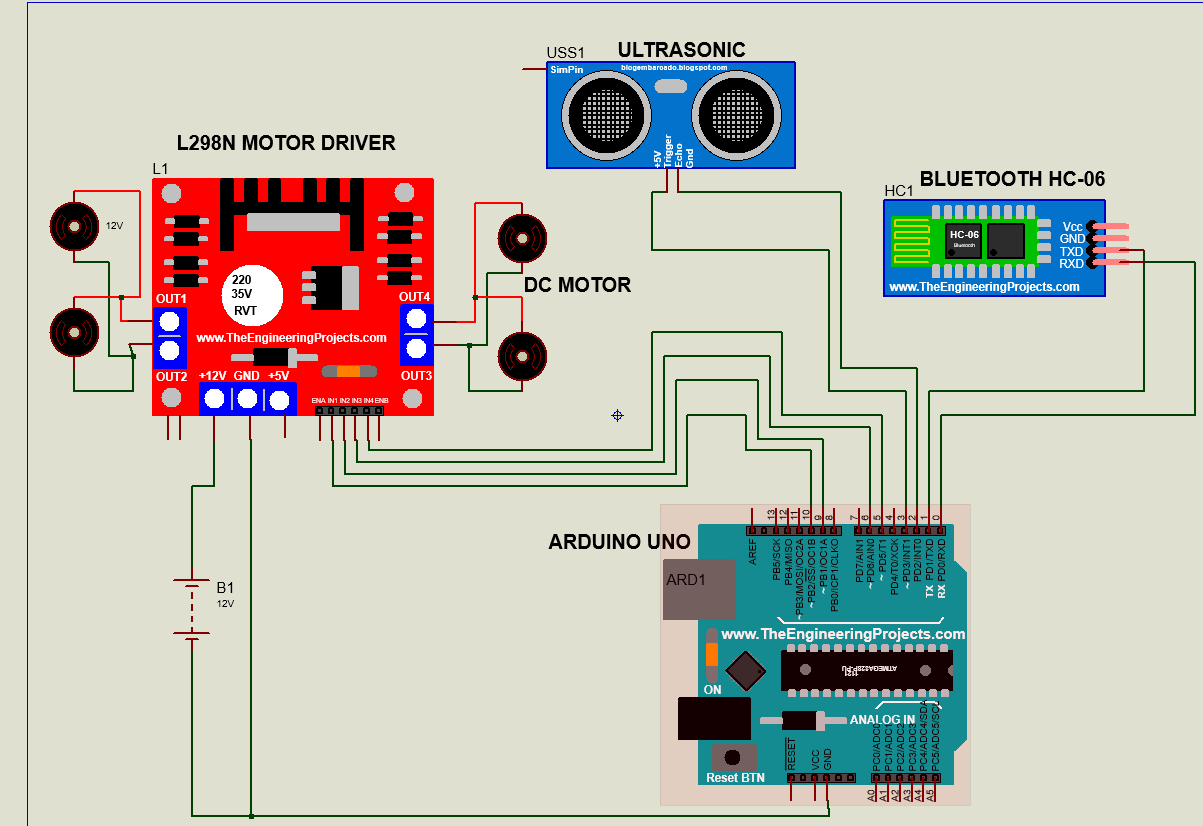
\includegraphics [width=1\textwidth,height=12cm]{Connictions.PNG}
    \caption{System Connections}
    \label{fig:Connections}
\end{figure}


%--[chapter4:RESULTS AND DISCUSSIONS]-
%__________________________________________________________________________________________________________________________________________________
\chapter{RESULTS AND DISCUSSIONS}
\section{\fontsize{12}{12}\selectfont{Results}}
In this chapter, we'll discuss the outcomes of our system's implementation.

The application starts with the main page that has a Bluetooth address and two buttons, as well as a Bluetooth address that displays the address of another Bluetooth device. The first button is MANUAL, which takes you to the manual driving page, and the second is the ADAS button, which takes you to the ADAS page.
\begin{figure}[H]
    \centering
    \graphicspath{ {./images/} }
    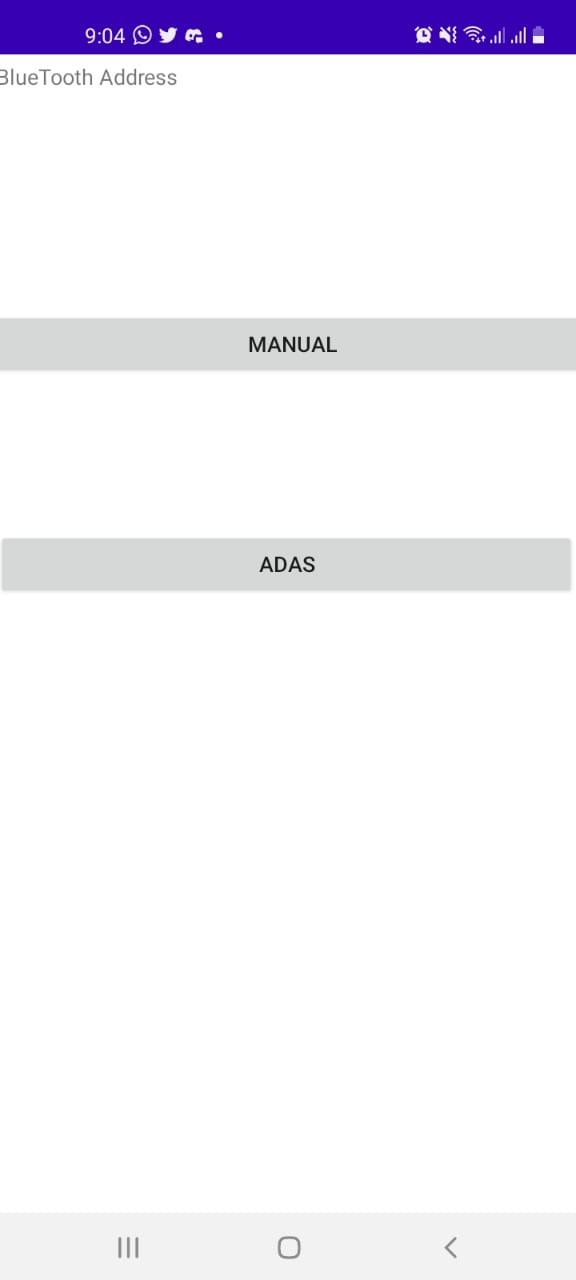
\includegraphics[width=.5\textwidth,height=.5\textheight ]{main.jpg}
    \caption{The main page}
    \label{fig:mesh1}
\end{figure}
On manual driving page, the user can manually drive the car in four directions (FORWARD, REVERSE, LEFT, RIGTE), as well as STOP, and can return to the main page by pressing the BACK TO MAIN button.
\begin{figure}[H]
    \centering
    \graphicspath{ {./images/} }
    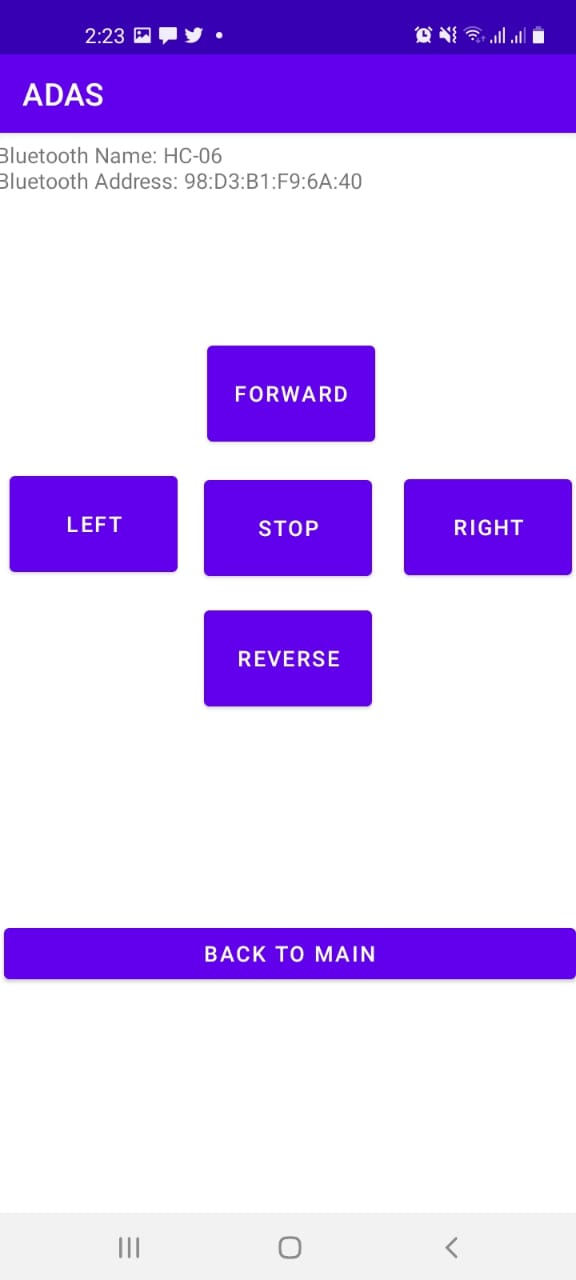
\includegraphics[width=.5\textwidth,height=.5\textheight ]{manual.jpg}
    \caption{The  manual driving page}
    \label{fig:mesh1}
\end{figure}
There are four buttons on the ADAS page. As indicated in the figure, each of these buttons takes you to a distinct system page (ACC system page, ESC system page, FCW system page, LDW system page). The ACC system is implemented in our application, therefore pressing the ACC system button takes the user to the ACC system page, and pressing the BACK TO MAIN button returns the user to the main page.
\begin{figure}[H]
    \centering
    \graphicspath{ {./images/} }
    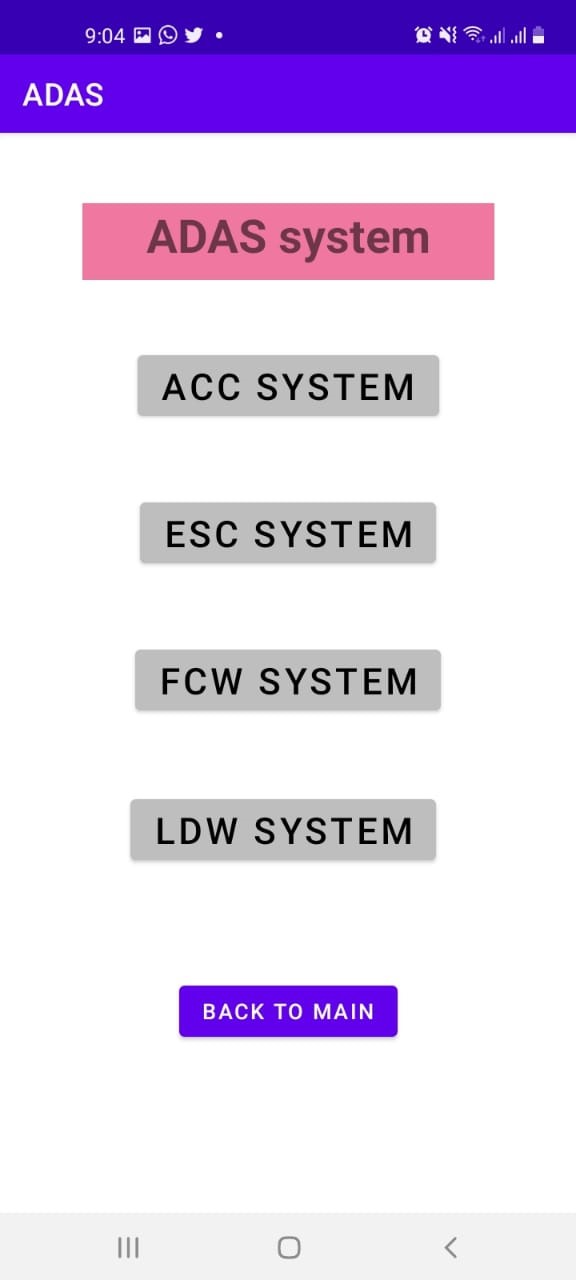
\includegraphics[width=.5\textwidth,height=.5\textheight ]{adas.jpg}
    \caption{ The ADAS page}
    \label{fig:mesh1}
\end{figure}
On the ACC system page, the user can enter the initial speed that the car should move at when the ACC system is active. The user presses the SEND button, then the START button to start the ACC system. The user can stop the system by pressing the STOP button.  and the user can press the BACK TO MAIN button to return to the main page or the BACK TO ADAS button to return to the ADAS page.
\begin{figure}[H]
    \centering
    \graphicspath{ {./images/} }
    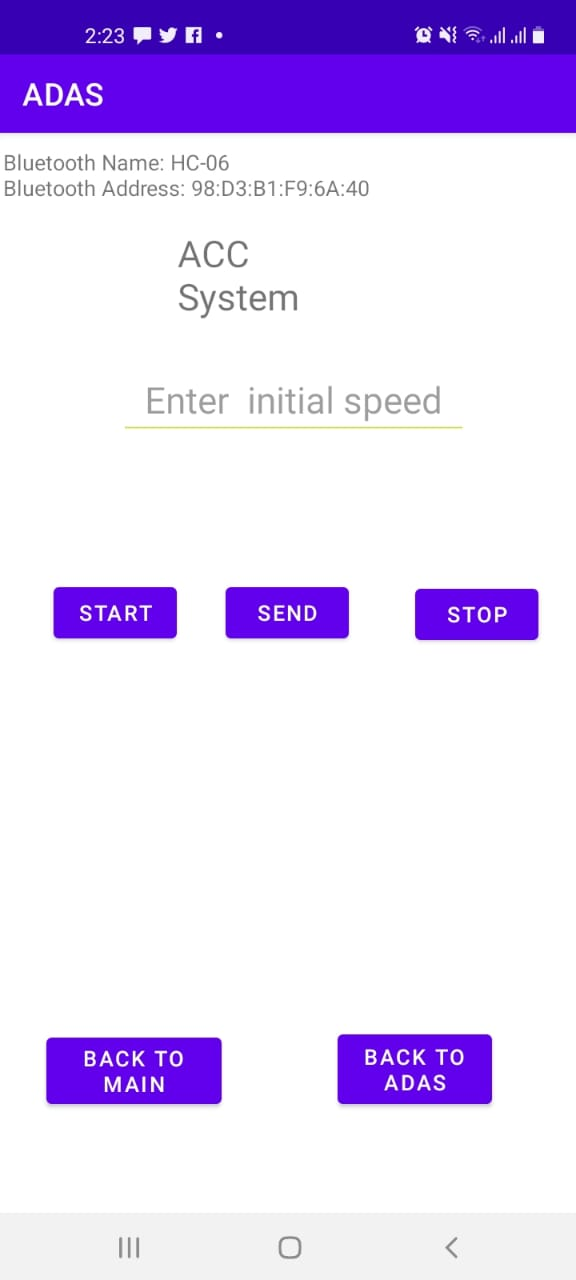
\includegraphics[width=.5\textwidth,height=.5\textheight ]{acc.jpg}
    \caption{ The ACC page}
    \label{fig:mesh1}
\end{figure}
In our system, if the user selects the manual drive, the wheels move in the same direction as the user selects in the application, and if the user selects the ACC system, the car will move at the initial speed that the user specific in the application. Then the ultrasonic measures the front distance (D). if the D$>=$ D1 cm the car keeps moving in the initial speed. else if   DS$<$D$<$D1 cm the speed will be gradually decreased. If the D$<$ DS it’s the stop distance, so the car will stop.
\begin{figure}[H]
    \centering
    \graphicspath{ {./images/} }
    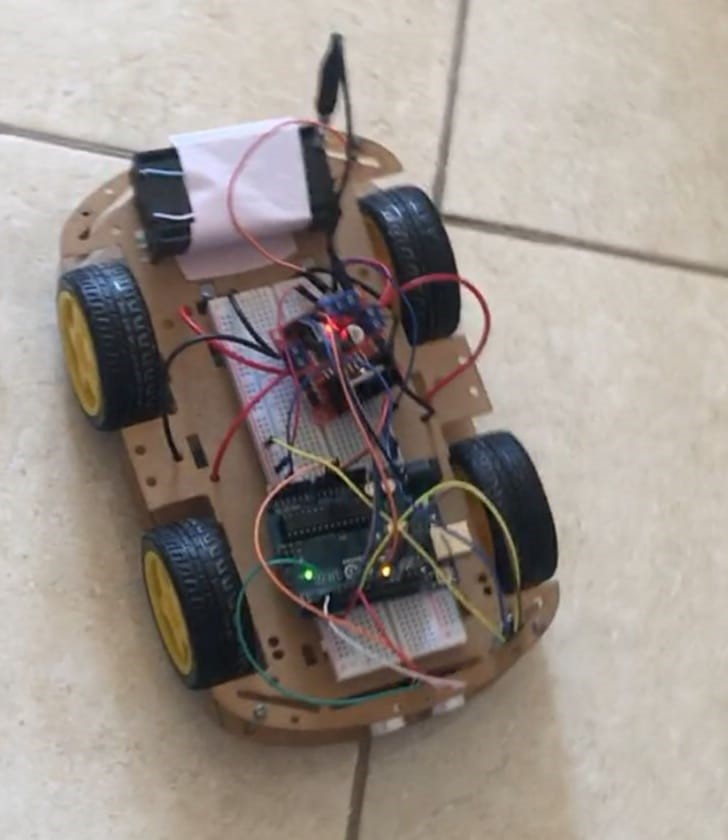
\includegraphics[width=.5\textwidth,height=.5\textheight ]{final.jpg}
    \caption{ The final form of the car}
    \label{fig:mesh1}
\end{figure}

\section{\fontsize{12}{12}\selectfont{Discussions}}
 Our project meets the main goal of implementing the ACC system to regulate the speed based on the measurement of front distance, so the speed will be reduced to keep the distance between the cars safe, and the user can manage the car using the application. based on the results in the previous section.
However, because we use the Bluetooth module and the wifi is costly, and 3G and 4G networks are not available in Palestine, there is some latency while transmitting commands via the application.


%--[chapter5:PROJECT MANAGEMENT]------------------------------------------------------------------------------------------------------------------------

\chapter{PROJECT MANAGEMENT}
\section{\fontsize{12}{12}\selectfont{Tasks, Schedule and Milestones}}

\begin{figure}[H]
    \centering
    \graphicspath{ {./images/} }
    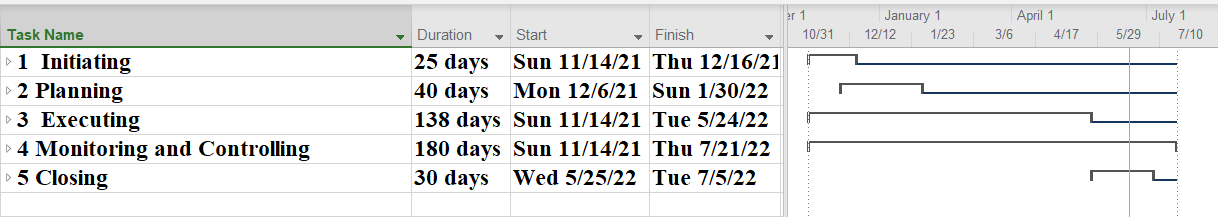
\includegraphics[width=1\textwidth,height=0.12\textheight]{Gantt chart-0.png}
    \caption{Gantt chart-0}
    \label{fig:Gantt-0}
\end{figure}
%-0
\begin{figure}[H]
    \centering
    \graphicspath{ {./images/} }
    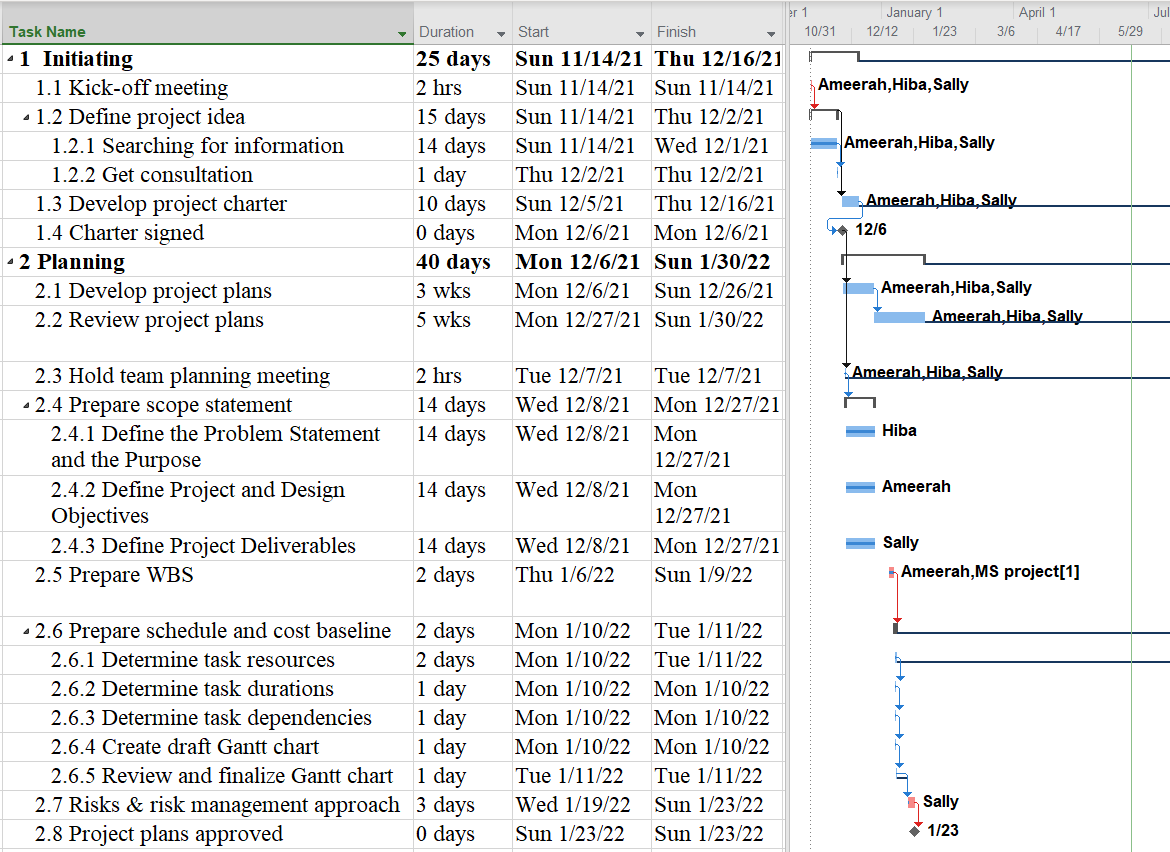
\includegraphics[width=1\textwidth,height=0.4\textheight]{Gantt chart-1.png}
    \caption{Gantt chart-1}
    \label{fig:Gantt-1}
\end{figure}
%-1
\begin{figure}[H]
    \centering
    \graphicspath{ {./images/} }
    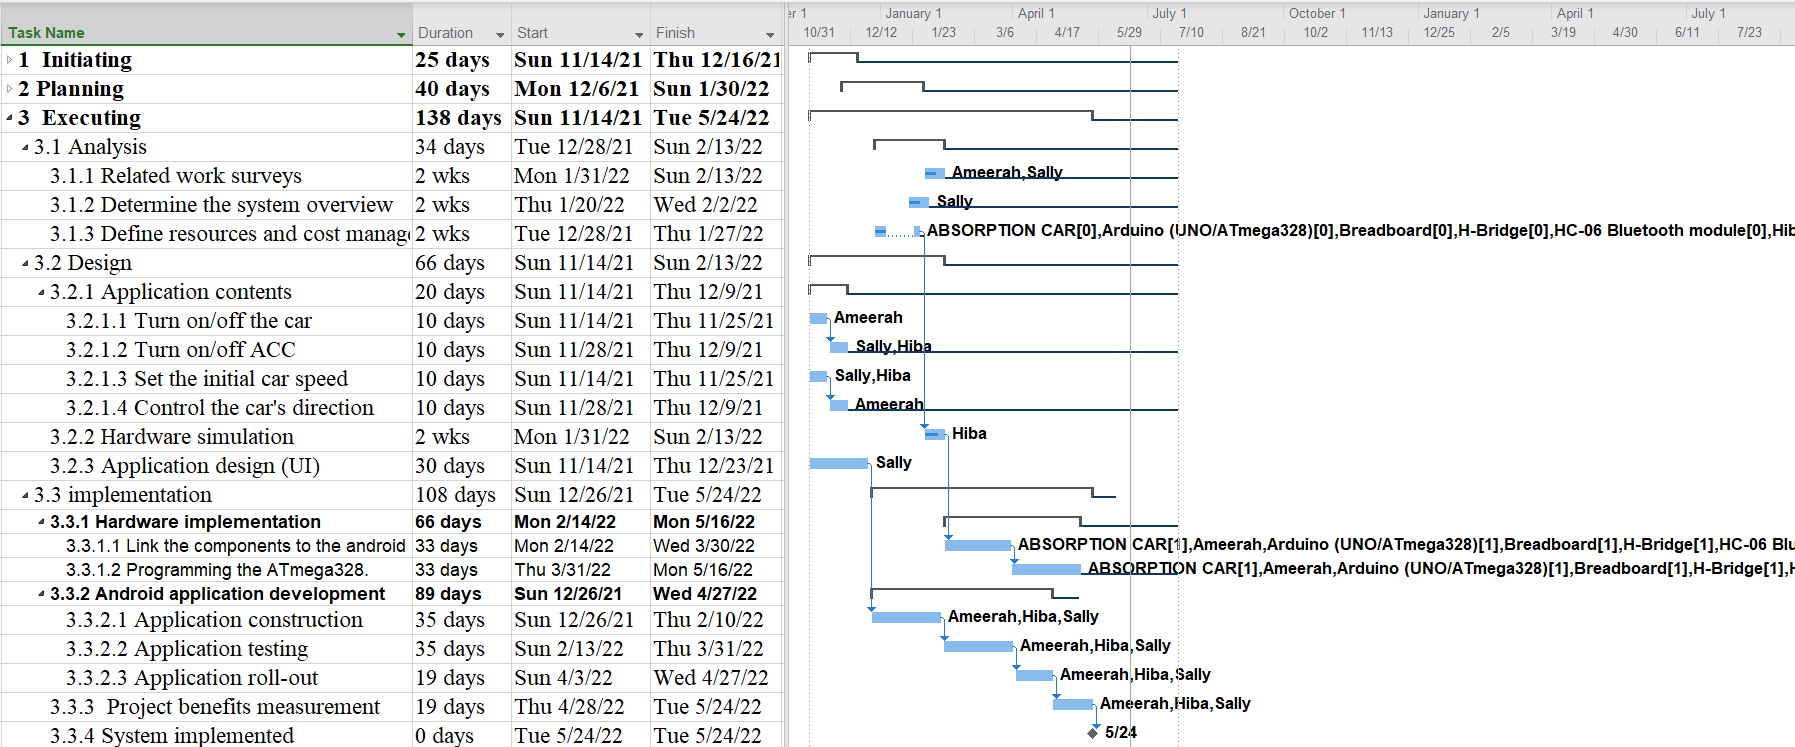
\includegraphics[width=1\textwidth,height=0.4\textheight]{Gantt chart-2.png}
    \caption{Gantt chart-2}
    \label{fig:Gantt-2}
\end{figure}
%-2
\begin{figure}[H]
    \centering
    \graphicspath{ {./images/} }
    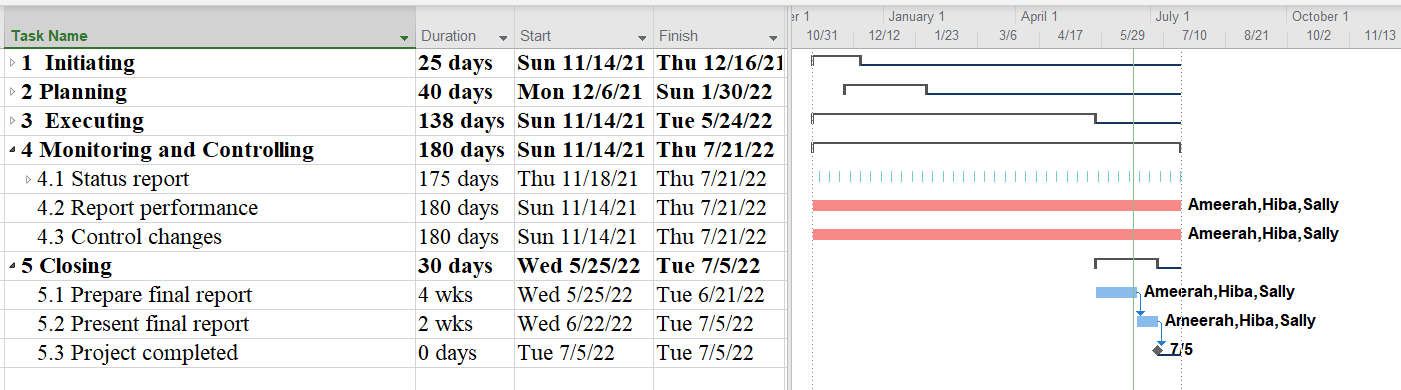
\includegraphics[width=1\textwidth,height=0.4\textheight]{Gantt chart-3.png}
    \caption{Gantt chart-3}
    \label{fig:Gantt-3}
\end{figure}
%section{Resources and Cost Management}
\section{\fontsize{12}{12}\selectfont{Resources and Cost Management}}

\begin{table}[H]
\begin{center}
\caption{Total cost of senior project items}
\label{tab:Table1}  
\begin{tabular}{|p{6cm}  |p{1cm}  |p{2cm}  |p{1.7cm} |p{3.5cm}|}

\hline
\begin{center}
\textbf{Item} 
\end{center}

& \begin{center}
\textbf{\#Unit }
\end{center}

& \begin{center}
\textbf{Unit Cost(\$)}
\end{center}

&\begin{center}
 \textbf{Subtotals}
\end{center}

& \begin{center}
\textbf{Comments}
\end{center}

 \\ 



\hline
\begin{center} Arduino(UNO/ATmega328)    \end{center}  &\begin{center}1 \end{center} & \begin{center} 15 \end{center}	& \begin{center} 15	\end{center}     &	 \\\hline


\begin{center} Ultrasonic Sensor  \end{center}  &\begin{center}1 \end{center} & \begin{center} 6 \end{center}	& \begin{center} 6	\end{center}     &	 \\\hline


\begin{center} HC-06 Bluetooth module   \end{center}  &\begin{center}1 \end{center} & \begin{center} 9 \end{center}	& \begin{center} 9	\end{center}     &	 \\\hline


\begin{center} Car   \end{center}  &\begin{center}1 \end{center} & \begin{center} 45 \end{center}	& \begin{center} 45	\end{center}     &	 \\\hline


\begin{center} Motor driver    \end{center}  &\begin{center}2 \end{center} & \begin{center} 8\end{center}	& \begin{center} 16	\end{center} &In our project, one motor driver was used, but the second was purchased as a replacement for the first one that was damaged.
\\\hline


\begin{center} Battery    \end{center}  &\begin{center}2 \end{center} & \begin{center} 9 \end{center}	& \begin{center} 18	\end{center}     &	 \\\hline


\begin{center} Charger	    \end{center}  &\begin{center}1 \end{center} & \begin{center} 12 \end{center}	& \begin{center} 12	\end{center}     &	 \\\hline


\begin{center} Breadboard	    \end{center}  &\begin{center}1 \end{center} & \begin{center} 5 \end{center}	& \begin{center} 5	\end{center}     &	 \\\hline


\begin{center} Wires	    \end{center}  &\begin{center}2 \end{center} & \begin{center} 6 \end{center}	& \begin{center} 12	\end{center}     &	 \\\hline




Total senior project estimate:  &\multicolumn{4}{c|}{138 \$}	\\\hline
\end{tabular}
\end{center}  
\end{table}




%\section{Lessons Learned} 
\section{\fontsize{12}{12}\selectfont{Lessons Learned}}
From working on the senior project, we've learned some constructive practices, such as working as a team, sharing tasks evenly, and cooperating to solve any problems that arise. One of the most critical aspects of a project's success is its advance preparation. Studying prior projects and learning from their mistakes in order to work on solving similar problems that may arise in our project and correctly managing it. Calculate the amount of time needed to complete the job and stick to the deadlines.
However, there were some drawbacks to working on the graduation project, such as the fact that not all of the components were available in our city, requiring a lot of effort; the hardware parts were affected by external factors, necessitating the purchase of some components again; and there were some problems and errors during programming that took a long time to resolve.

%-
%--[chapter6:IMPACT OF THE ENGINEERING SOLUTION]------------------------------------------------------------------------------------------------------------------------

\chapter{IMPACT OF THE ENGINEERING SOLUTION}
\section{\fontsize{12}{12}\selectfont{Economical, Societal and Global}}
The increasing number of accidents is one of the major drivers responsible for the growth of adaptive cruise control systems. So, there has been a continuous demand for increasing safety features to be installed during the manufacturing of vehicles. The ACC system will reduce the number of accidental deaths and injuries. An adaptive cruise control system will help to control the speed of vehicles and maintain a safe distance between two vehicles. 
The increase in demand for adaptive cruise control systems in the global market is because of the rising number of accidents due to an increase in traffic. Another reason is increasing incomes and greater sales of luxury cars. And increasing using sensors with the another technology.
It also saves you money by increasing your gas mileage and thus minimizing your vehicle's fuel consumption.Also Because it's easier to keep inside the speed limit, there are fewer speeding tickets.


\section{\fontsize{12}{12}\selectfont{Environmental and Ethical}}
The usefulness of a system is directly proportional to its use in the correct recommended manner. The system should be used in straight or fast ways and avoided on slopes. Using the system does not mean that the driver is not responsible for driving, there are situations that require quick intervention from the driver.
The goal of the system, if used in the correct way, is to reduce driver fatigue over long distances and reduce traffic accidents resulting from collision between cars or a car hitting a fixed barrier, run-over accidents, as well as contribute to the regulation of traffic.
The system contributes to saving lives and enhancing safety while driving. Thus, it can be said that the project has a positive ethical and environmental impact.



%--[chapter7:CONCLUSIONS AND RECOMMENDATIONS]-
\chapter{CONCLUSIONS AND RECOMMENDATIONS}

\section{\fontsize{12}{12}\selectfont{Summary of Achievements of the Project Objectives}}
The main objective of our project to design a system that helps reduce traffic accidents. Indeed, after continuous and intense work for a period of time, we were able to achieve the desired goal. The system is designed and built according to the planned requirements. A mobile application is created to control the vehicle's motion and the ACC system through commands that are sent to the control unit via the Bluetooth module. Despite the challenges we faced, such as the lack of required components and a defect in the internal installation of some components, we were able to complete the project at the lowest possible cost and on time. This was a very useful experience for us we learned to work within one team to reach our common goal on time.

\section{\fontsize{12}{12}\selectfont{New Skills and Experiences Learnt}}
This experience and project provided us with a wealth of knowledge and skills that will serve us well in the future, particularly in our profession. For example, we learned new skills like latex, Android development, and Arduino, which we used to create the Android application that control the overall system. We also improved our knowledge of the Java programming language, which we used to create the Android application. We also learned how to connect the hardware and link it to the software (application).


\section{\fontsize{12}{12}\selectfont{Recommendations for Future Work}}
We will discuss some of the future features that can be added to the system. These features will improve system functionality. The ability to connect via 3G and 4G networks could be added to the system in the future. Furthermore, the ACC's behavior improved on non-straight roads, particularly roundabouts, up and down hills, and in windy conditions. integrating ACC with other ADAS assistance systems, such as automatic parking, which assists in moving the vehicle from a traffic lane to a parking space, and a car navigation system, which assists in finding direction in an automobile.

\bibliographystyle{plain}
\bibliography{References}

\chapter*{APPENDICES} 
\addcontentsline{toc}{chapter}{APPENDICES}
\subsection*{Appendix A:}
\addcontentsline{toc}{subsection}{Appendix A:}
{\large Arduino code for Manual driving :}

char t;\\
\#include$<$SoftwareSerial.h$>$ \\
SoftwareSerial mySerial(8, 9); // RX | TX \\
int IN1 = 11;\\
int IN2 = 10;\\
int IN3 = 6;\\
int IN4 = 5;\\
void setup() \{\\
// put your setup code here, to run once:\\
  pinMode(IN1, OUTPUT);\\
  pinMode(IN2, OUTPUT);\\
  pinMode(IN3, OUTPUT);\\
  pinMode(IN4, OUTPUT);\\
  digitalWrite(IN1, LOW);\\
  digitalWrite(IN2, LOW);\\
  digitalWrite(IN3, LOW);\\
  digitalWrite(IN4, LOW);\\
  mySerial.begin(9600);\\
  Serial.begin(9600);\\
\}\\
void loop() \{\\
  // put your main code here, to run repeatedly:\\
  if (mySerial.available())\{// print from phone\\
    t =mySerial.read();\\
    Serial.print(t);\}\\ 
  else if (Serial.available()) \{ // print to phone\\
    t = Serial.read();\\
    mySerial.println(t);\\
  \} \\
if(t == 'B')\{            //move forward(all motors rotate in forward direction)\\
  analogWrite(IN1, 100);\\
  analogWrite(IN2, 0);\\
  analogWrite(IN3, 100);\\
  analogWrite(IN4, 0);\\
\}\\
else if(t == 'F')\{      //move reverse (all motors rotate in reverse direction)\\
  analogWrite(IN1, 0);\\
  analogWrite(IN2, 100);\\
  analogWrite(IN3, 0);\\
  analogWrite(IN4, 100);\\
\}\\
else if(t == 'L')\{      //turn right (left side motors rotate in forward direction, right side motors doesn't rotate)\\
  analogWrite(IN1, 0);\\
  analogWrite(IN2, 0);\\
  analogWrite(IN3, 0);\\
  analogWrite(IN4, 100);\\
\}\\
else if(t == 'R')\{      //turn left (right side motors rotate in forward direction, left side motors doesn't rotate)\\
   analogWrite(IN1, 0);\\
  analogWrite(IN2, 100);\\
  analogWrite(IN3, 0);\\
  analogWrite(IN4, 0);\\
\}\\
else if(t == 'S')\{      //STOP (all motors stop)\\
  analogWrite(IN1, 0);\\
  analogWrite(IN2, 0);\\
  analogWrite(IN3, 0);\\
  analogWrite(IN4, 0);\\
\}\\
\}\\

{\large Arduino code for AAC system :}

char t;\\
String content = "";\\
int intial=0;\\
\#include$<$SoftwareSerial.h$>$ \\
SoftwareSerial mySerial(8, 9); // RX | TX\\
int IN1 = 11;\\
int IN2 = 10;\\
int IN3 = 6;\\
int IN4 = 5;\\
float d1=100,ds=20;\\
int pulse; //from sinsor\\
float d=0;// distance in cm\\
//Function to get distance from snisor\\
float readUltrasonicDistance(int triggerPin, int echoPin)\\
\{\\
  digitalWrite(triggerPin, LOW);\\
  delayMicroseconds(20);\\
  digitalWrite(triggerPin, HIGH);\\
  delayMicroseconds(100);\\
  digitalWrite(triggerPin, LOW);\\
  pulse = pulseIn(echoPin, HIGH);\\
  return pulse / 29.387 / 2;\\
\}//end readUltrasonicDistance\\

void keepLimit(int s)\\
\{\\
    analogWrite(IN2,s);//11\\
    analogWrite(IN4,s);//6\\
\}//end of keepLimit\\

void reduce(int s)\\
\{\\
    analogWrite(IN2,s/2);//11\\
    analogWrite(IN4,s/2);//6\\
\}//end of keepLimit\\
  
void Stop()\\
\{ \\
    analogWrite(10, 0);\\
    analogWrite(11, 0);\\
    analogWrite(5, 0);\\
    analogWrite(6, 0);\\
    Serial.println("Stop()");\\
    delay(5000);\\
    loop();\\
\}//end of stop\\

void setup() \{\\
  Serial.println("setup");\\
  pinMode(3, INPUT);//Echo //3\\
  pinMode(2, OUTPUT);//trig //2\\
  pinMode(IN1, OUTPUT);\\
  pinMode(IN2, OUTPUT);\\
  pinMode(IN3, OUTPUT);\\
  pinMode(IN4, OUTPUT);\\
  mySerial.begin(9600);\\
  Serial.begin(9600);\\
\}\\
void loop() \{\\
Serial.println("loop");\\
 if (mySerial.available()){// print from phone\\
    t =mySerial.read();\\
    Serial.print(t);\\
    \ }\\
    if(t=='A')\{\\
    if (mySerial.available()){// print from phone\\
    content=mySerial.readString();\\
    intial=content.toInt(); \\
    Serial.println(intial);\\
    delay(3000); \}\\
    \}\\ 
  while( t!='S'  )\{\\
    if (mySerial.available()){// print from phone
    t =mySerial.read();\\
    Serial.print(t);}\\
    d = readUltrasonicDistance(2, 3);\\
    Serial.println(d);\\
    delay(200);\\
    if (d$>$d1)\{\\
    keepLimit(intial);\}\\
    else  if (ds$<$d$<$d1)\{\\
    reduce(intial);\\
    \} \\ 
   if (d $<$ ds) \{ \\ 
   t='S';\\
   break;\\
  \}\\
  \}//end while\\
   Stop();\\
  \}//end void loop()\\

  


\subsection*{Appendix B:}
\addcontentsline{toc}{subsection}{Appendix B:}

{\large Android code for Manual driving:}\\

package com.example.a;\\
import androidx.appcompat.app.AppCompatActivity;\\
import android.os.Bundle;\\
import java.io.IOException;\\
import java.util.Set;\\
import java.util.UUID;\\
import android.annotation.SuppressLint;\\
import android.app.Activity;\\
import android.bluetooth.BluetoothAdapter;\\
import android.bluetooth.BluetoothDevice;\\
import android.bluetooth.BluetoothSocket;\\
import android.content.Intent;\\
import android.graphics.Color;\\
import android.os.Bundle;\\
import android.view.MotionEvent;\\
import android.view.View;\\
import android.view.View.OnClickListener;\\
import android.widget.Button;\\
import android.widget.TextView;\\
import android.widget.Toast;\\
public class MainActivity extends Activity implements OnClickListener {

    Button forward\_btn, left\_btn, right\_btn,\\  
     reverse\_btn,stop\_btn,go\_to\_Manual;\\
    TextView t1;\\
    String address = null , name=null;\\
    BluetoothAdapter myBluetooth = null;\\
    BluetoothSocket btSocket = null;\\
    Set<BluetoothDevice> pairedDevices;\\
    static final UUID myUUID =\\
     UUID.fromString("00001101-0000-1000-8000-00805F9B34FB");\\
    \@Override\\
    protected void onCreate(Bundle savedInstanceState)\\
    \{\\
        super.onCreate(savedInstanceState);\\
        setContentView(R.layout.activity\_main);\\\
        go\_to\_Manual=findViewById(R.id.go\_to\_Manual);\\
        try {setw();} catch (Exception e) \{\}\\
    \}\\
    public void goAdas(View v)\{\\
        Intent intent=new Intent(MainActivity.this,adas.class);\\
        startActivity( intent );\\
    \}\\
    \@SuppressLint("ClickableViewAccessibility")\\
    private void setw() throws IOException\\
    \{\\
        t1=(TextView)findViewById(R.id.textView1);\\
        bluetooth\_connect\_device();\\
        go\_to\_Manual=(Button) findViewById(R.id.go\_to\_Manual);\\
        go\_to\_Manual.setOnTouchListener(new View.OnTouchListener()\\
        \{ \@Override\\
        public boolean onTouch(View v, MotionEvent event)\{\\
            if(event.getAction() == MotionEvent.ACTION\_UP){Send("M");\}\\
            return true;\}\\
       \});\\

        forward\_btn = (Button) findViewById(R.id.forward\_btn);\\
        forward\_btn.setOnTouchListener(new View.OnTouchListener()\\
        \{   \@Override\\
        public boolean onTouch(View v, MotionEvent event)\{\\
            if(event.getAction() == MotionEvent.ACTION\_UP){Send("F");\}\\
            return true;\}\\
        \});\\
        left\_btn =  (Button)findViewById(R.id.lef\_btn);\\
        left\_btn.setOnTouchListener(new View.OnTouchListener()\\
        \{   \@Override
        public boolean onTouch(View v, MotionEvent event)\{\\
            if(event.getAction() == MotionEvent.ACTION\_UP){Send("L");\}\\
            return true;\}\\
       \});\\
        reverse\_btn = (Button) findViewById(R.id.reverse\_btn);
        reverse\_btn.setOnTouchListener(new View.OnTouchListener()\\
        \{   \@Override\\
        public boolean onTouch(View v, MotionEvent event)\{\\
            if(event.getAction() == MotionEvent.ACTION\_UP){Send("B");\}\\
            return true;\}\\
        \});\\
        right\_btn = (Button) findViewById(R.id.right\_btn);\\
        right\_btn.setOnTouchListener(new View.OnTouchListener()\\
       \{   \@Override\\
        public boolean onTouch(View v, MotionEvent event)\{\\
            if(event.getAction() == MotionEvent.ACTION\_UP){Send("R");\}\\
            return true;\}\\
        \});\\
        stop\_btn = (Button) findViewById(R.id.stop\_btn);\\
        stop\_btn.setOnTouchListener(new View.OnTouchListener()\\
        \{   \@Override\\
        public boolean onTouch(View v, MotionEvent event)\{\\
            if(event.getAction() == MotionEvent.ACTION\_UP){Send("S");\}\\
            return true;\}\\
        \});\}\\

\ @SuppressLint("MissingPermission")\\
    private void bluetooth\_connect\_device() throws IOException\\
    \{\\
        try\\
        \{\\
            myBluetooth = BluetoothAdapter.getDefaultAdapter();\\
            address = myBluetooth.getAddress();\\
            pairedDevices = myBluetooth.getBondedDevices();\\
            if (pairedDevices.size()>0)\\
            \{\\
                for(BluetoothDevice bt : pairedDevices)\\
                \{\\
                    address=bt.getAddress().toString();name =\\
                     bt.getName().toString();\\
                    Toast.makeText(getApplicationContext(),"Connected",\\
                     Toast.LENGTH\_SHORT).show();\}\}\} \\
        catch(Exception we)\{\}\\
        myBluetooth = BluetoothAdapter.getDefaultAdapter();\\
        //get the mobile bluetooth device\\
        BluetoothDevice dispositivo =myBluetooth.getRemoteDevice(address);\\
         //connects to the device's address and checks if it's available\\
        btSocket = dispositivo.createInsecureRfcommSocketToServiceRecord(myUUID);\\
        //create a RFCOMM (SPP) connection\\
        btSocket.connect();\\
        try { t1.setText("Bluetooth Name: "name"Bluetooth Address:"address);\\
         \}\\
        catch(Exception e)\{\}\\
    \}\\
    public void onClick(View v)\\
    \{\\
        try\{\}\\
        catch (Exception e)\\
        \{\\
            Toast.makeText(getApplicationContext(),\\
            e.getMessage(), Toast.LENGTH\_SHORT).show();\}\}\\
    private void Send(String i)\{\\
     try\{\\
         if (btSocket!=null)\{\\
             btSocket.getOutputStream().write(i.toString().getBytes());
            \}\}\\
        catch (Exception e)
        \{\\
            Toast.makeText(getApplicationContext()\\
            ,e.getMessage(), Toast.LENGTH\_SHORT).show();\\

        \}\}\}\\
       

\subsection*{Appendix C:}
\addcontentsline{toc}{subsection}{Appendix C:}
        
{\large Android code for ACC system:}\\

package com.example.a;\\
import androidx.appcompat.app.AppCompatActivity;\\
import android.os.Bundle;\\
import java.io.IOException;\\
import java.util.Set;\\
import java.util.UUID;\\
import android.annotation.SuppressLint;\\
import android.app.Activity;\\
import android.bluetooth.BluetoothAdapter;\\
import android.bluetooth.BluetoothDevice;\\
import android.bluetooth.BluetoothSocket;\\
import android.content.Intent;\\
import android.graphics.Color;\\
import android.os.Bundle;\\
import android.view.MotionEvent;\\
import android.view.View;\\
import android.view.View.OnClickListener;\\
import android.widget.Button;\\
import android.widget.TextView;\\
import android.widget.Toast;\\
public class acc  extends AppCompatActivity  implements OnClickListener \{\\
    Button go\_to\_Manual; \\
    Button Start\_Acc,Stop\_Acc,Display\_speed,Send; \\
    TextView Speed,Speed2;\\
    TextView t1;\\
    String address = null , name=null;\\
    BluetoothAdapter myBluetooth = null;\\
    BluetoothSocket btSocket = null;\\
    Set<BluetoothDevice> pairedDevices;\\
    static final UUID myUUID =    \\ 
    UUID.fromString("00001101-0000-1000-8000-00805F9B34FB");\\
    \@Override\\
    protected void onCreate(Bundle savedInstanceState)\\
    \{\\
        super.onCreate(savedInstanceState);\\
        setContentView(R.layout.activity\_acc);\\
        go\_to\_Manual=findViewById(R.id.go\_to\_Manual);\\
        Start\_Acc=findViewById(R.id.start);\\
        Send=findViewById(R.id.send);\\
        Speed=findViewById(R.id.speed);\\
        Speed2=findViewById(R.id.speed2);\\
        try \{setw();\} catch (Exception e)\{\}\\
       
    \} //end onCreate\\
    public void back\_adas(View v)\{\\
        Intent intent=new Intent(acc.this,adas.class);\\
        startActivity( intent );\\
   \ }\\
    public void acc\_To\_manual(View v)\{\\
        Intent intent=new Intent(acc.this,MainActivity.class);\\
        startActivity( intent );\\
    \}\\
    \@SuppressLint("ClickableViewAccessibility")\\
     private void setw() throws IOException\\
    \{\\
        t1=(TextView)findViewById(R.id.textView1);\\
        bluetooth\_connect\_device();\\
        Send= (Button) findViewById(R.id.send);\\
        Send.setOnTouchListener(new View.OnTouchListener()\\
        \{   @Override\\
        public boolean onTouch(View v, MotionEvent event)\{\\
            if(event.getAction() == MotionEvent.ACTION\_UP)  
             \{Send(Speed.getText().toString());\}\\
              return true;\}\\
        \});\\
        Start\_Acc= (Button) findViewById(R.id.start);\\
        Start\_Acc.setOnTouchListener(new View.OnTouchListener()\\
       \{   @Override\\
        public boolean onTouch(View v, MotionEvent event)\{\\
            if(event.getAction() == MotionEvent.ACTION\_UP){Send("A");\}\\
            return true;\}\\
        });\\
        Stop\_Acc= (Button) findViewById(R.id.stop);\\
        Stop\_Acc.setOnTouchListener(new View.OnTouchListener()\\
        \{   @Override\\
        public boolean onTouch(View v, MotionEvent event)\{\\
            if(event.getAction() == MotionEvent.ACTION\_UP){Send("S");}
            return true;\}\\
        \});\\

       \}\\
   \ @SuppressLint("MissingPermission")\\
    private void bluetooth\_connect\_device() throws IOException\\
    \{\\
        try\\
        \{\\
            myBluetooth = BluetoothAdapter.getDefaultAdapter();\\
            address = myBluetooth.getAddress();\\
            pairedDevices = myBluetooth.getBondedDevices();\\
            if (pairedDevices.size()>0)\\
            \{\\
                for(BluetoothDevice bt : pairedDevices)\\
                \{\\
                    address=bt.getAddress().toString();name =\\
                     bt.getName().toString();\\
                    Toast.makeText(getApplicationContext(),"Connected",\\
                     Toast.LENGTH\_SHORT).show();\}\}\} \\
        catch(Exception we)\{\}\\
        myBluetooth = BluetoothAdapter.getDefaultAdapter();\\
        //get the mobile bluetooth device\\
        BluetoothDevice dispositivo =myBluetooth.getRemoteDevice(address);\\
         //connects to the device's address and checks if it's available\\
        btSocket = dispositivo.createInsecureRfcommSocketToServiceRecord(myUUID);\\
        //create a RFCOMM (SPP) connection\\
        btSocket.connect();\\
        try { t1.setText("Bluetooth Name: "name"Bluetooth Address:"address);\\
         \}\\
        catch(Exception e)\{\}\\
    \}\\
    public void onClick(View v)\\
    \{\\
        try\{\}\\
        catch (Exception e)\\
        \{\\
            Toast.makeText(getApplicationContext(),\\
            e.getMessage(), Toast.LENGTH\_SHORT).show();\}\}\\
    private void Send(String i)\{\\
     try\{\\
         if (btSocket!=null)\{\\
             btSocket.getOutputStream().write(i.toString().getBytes());
            \}\}\\
        catch (Exception e)
        \{\\
            Toast.makeText(getApplicationContext()\\
            ,e.getMessage(), Toast.LENGTH\_SHORT).show();\\

        \}\}\}\\

  














\end{document}
